\documentclass[UTF8, 12pt]{article}

\usepackage{ctex}
\usepackage{inputenc}
\usepackage{amsmath}
\usepackage[margin=1in]{geometry}
\usepackage{graphicx}
\usepackage[colorlinks=true, linkcolor=red, urlcolor=blue]{hyperref}
\usepackage{xcolor}
\usepackage{tikz}
\usepackage{pgfplots}
\usepackage{float}
\usepackage{amsmath}
\usepackage{amssymb}

\usepackage{tcolorbox} % box制作基本宏包
\usepackage{varwidth} % box宽度设置需要
\usepackage{ruby} % 标注

\usepackage{enumitem} % 列表宏包
\usepackage{listings} % 代码宏包
\usepackage{minted}

\tcbuselibrary{breakable} %box内自动折行
\tcbuselibrary{skins} % 填充等

\usetikzlibrary{arrows.meta}
\pgfplotsset{compat=1.18}

\tcbset{
    myrecommendbox/.style={
        colback=yellow!10!white,
        colframe=yellow!50!black,
        fonttitle=\bfseries,
        coltitle=black,
        colbacktitle=yellow!50!white,
        boxrule=0.5mm,
        arc=4mm,
        outer arc=4mm,
        boxsep=5pt,
        left=5pt,
        right=5pt,
        top=5pt,
        bottom=5pt,
        breakable,
        enhanced,
    }
}
\newcommand{\emptyline}{\vspace{\baselineskip}}
\newcommand{\uhref}[2]{\,\href{#1}{\,\underline{#2}}\,}
\newcommand{\uurl}[1]{\,\href{#1}{\,\underline{#1}}\,}

\newcommand{\textoverset}[2]{$\overset{\text{#1}}{\text{#2}}$}

\newcommand{\bfx}{{\mathbf{x}}}
\newcommand{\bfy}{{\mathbf{y}}}
\newcommand{\bfr}{{\mathbf{r}}}

\DeclareMathOperator*{\argmin}{arg\,min}

\title{如何理解神经网络——信息量、压缩与智能}
\author{gtj}
\date{\today}

\begin{document}

\maketitle

\tableofcontents
\newpage

\section{从函数拟合开始}
% 引入拟合的基本思想
\subsection{最简单的规律——简单线性回归}

\begin{figure}[H]
    \centering
    \includegraphics[width=0.6\textwidth]{img/linear_regression.png}
    \caption{线性回归示意图}
    {图源: \uhref{https://en.wikipedia.org/wiki/Linear_regression}{Wikipedia}}
    \label{fig:linear_regression}
\end{figure}

虽然\textoverset{Linear Regression}{线性回归}的名字叫做“\textoverset{Regression}{回归}”,但是事实上我更喜欢叫做\textoverset{Linear Fitting}{线性拟合}。它的目的是找到一条直线尽可能“贴近”数据点。在这一基础上,我们可以发现数据之间的规律,从而做出一些预测。不过这里有几个问题:
\begin{itemize}
    \item 为什么要用直线?为什么不用曲线?
    \item 为什么要用直线拟合数据点?这有什么用?
    \item “贴近”数据点的标准是什么?为什么要选择这个标准?
\end{itemize}

我认为用直线的原因无非两点:一是直线 $y = kx+b$ 简单且意义明确,又能处理不少的问题。几何上直线作为基本对象,尺子就能画出;代数上只需要加减乘除,一次函数我们也很早就学过了。而它的思想一路贯穿到了微积分的导数并延申到了线性代数。二是许多曲线的回归可以转为线性回归(见后文)。例如指数型的 $y = k \mathrm{e}^{\alpha x}$ 取对数变为 $z = \alpha x + \ln k$,又如分式型的 $y = (\alpha x + \beta)^{-1}$ 取倒数转化为 $z = \alpha x + \beta$,从而归结为线性拟合。因此带着线性拟合经验再去考虑曲线会更轻松。

至于其意义:一是找到数据的规律,二是做出预测。拟合的系数可以用于测算数据之间的关系,斜率 $k$ 表明输出对输入的敏感程度。一个经典例子是广告投放的\textoverset{Marginal Benefit}{边际效益}\footnote{边际效益:经济学概念,每增加单位投入,产出会增加多少单位},在一定范围内拟合收益与投入的关系,可以估算当前的边际效益,从而决定是否继续投放。而物理上,比值定义法定义的各种物理量,如电阻、电容等,最常用的测算方式都是线性拟合。例如测量电源输出的若干组电压和电流数据,并拟合出直线,斜率的绝对值是电源的内阻,同时截距顺带给出了电源的电动势,这样测得的数据就可以用于预测电源的输出情况。对我们所处的世界有定量的认识是科学的基础。可测量的数据和数学模型来描述、解释和预测自然现象是科学的基本方法,也是拟合的根本目的。

既然有了基本思路,那么如何选择“贴近”的标准呢?直接去度量一堆散点和直线的接近程度多少有点霰弹枪\footnote{霰弹枪:一种枪,射出的子弹像雨点一样散开}打移动靶的感觉,但是我们总是可以计算子弹打到了几环。换言之,两个相差的部分才是关键的,\textoverset{Residual}{残差}的概念由此产生。取出每个点实际值和拟合值的差,就得到了这样一个列表\footnote{记号说明:对于变量,无论是一维变量还是多维变量,一律采用斜体。对于具体的数据点,视是否为向量决定使用黑体还是斜体。例如 $r = y - \hat y$ 表示的是方程,所以全部采用斜体。但是具体数据的残差计算,例如 $\bfr = \bfy - \hat \bfy$,是对数据点的向量运算,所以采用正体。}(其中根据拟合函数 $\hat y_i = kx_i + b$ 计算出预测值):
\[
    \bfr = [r_1, r_2, \ldots, r_n] = [y_1 - \hat y_1, y_2 - \hat y_2, \ldots, y_n - \hat y_n]
\]

度量数据点与直线间偏差这一问题就转为了度量残差与 0 的偏差。还记得勾股定理吗?直角坐标系内一点到 0 的距离是坐标平方和的平方根,只不过这里残差列表是个 $n$ 维的向量,度量它偏离原点的程度就是向量的\textoverset{Norm}{模}。这个模越小,说明拟合的效果越好。这样我们就自然地引入了度量拟合效果的量化标准,不过实际应用中出于方便(特别是计算上的方便),通常省去开根号的一步,直接采用残差的平方和,此外还会除以样本点数得到“平均”的残差平方。习惯上称之为\textoverset{Mean Squared Error}{均方误差}(MSE):
\[
    \text{MSE} = \frac1n |\bfr|^2 = \frac1n \sum_{i=1}^n r_i^2
\]

在踏出下一步之前,我想这里有一点点思考的空间。例如:
\begin{itemize}
    \item 为什么要用平方和而不是直接相加呢?

          这是因为直接相加会有正负相互抵消的可能,度量出的偏差为 0 甚至为负实在是不合理,因此至少要保证每一项都是正数。但是这又引出下一个问题。

    \item 为什么不用绝对值呢?绝对值也是正的啊。

          从正态分布的角度看,选用平方和自有它的\uhref{https://www.zhihu.com/question/20447622/answer/25186207}{道理}。但是即使读者并不熟悉这些统计的背景,也可以从另一个角度理解:平方和的确是一个更好的度量方式,因为它对大的偏差更加敏感。例如一个残差为 2 的点和一个残差为 4 的点,直接绝对值相加的话是 6,在这里残差为 4 的点贡献了 $4 / 6 \approx 66.7\%$ 的偏差。而它们的平方和是 $2^2 + 4^2 = 20$,残差为 4 的点贡献提升到了 $4^2 / 20 = 80\%$,更加凸显出了 4 的偏差,反映了我们更“关注”这一大偏差的想法,更符合通常对“偏差”的直观认识。

    \item 为什么要除以样本点数 $n$ 呢?

          一方面是为了跨数据集比较,数据集的大小通常有区别,就像买东西的重量。这正如不能光看价格不看质量就评价 5 元 2 斤的苹果贵还是 3 元 1 斤的苹果贵,因此需要一个“单位”来衡量。另一方面,看完下一个问题你就会明白其中的精妙之处。

    \item 这里直接把所有的残差平方加了起来,但如果有的点重要一些怎么办?

          先说明一下这样的需求并非空想,有时测量条件决定了不同点的可靠性并不相同。以一个精度 1\% 的表为例,测量得到 1.00, 2.00, 3.00 时它们本身允许的误差分别是 0.01, 0.02, 0.03,而非相同。也就是说我们会觉得 1.00 的测量值从残差的大小上\footnote{残差的大小:严谨的说称作\textoverset{Absolute Error}{绝对误差}}更为可靠,这时似乎应该衡量一下点的“重要性”。如果你想说一个点很重要怎么办?直观上来讲你可能会想把它重复几遍,例如如果你很关心 $r_1$,你可能会想,这还不简单吗?在误差列表中把 $r_1$ 重复 3 遍就好,就像这样:
          \[
              \text{Refined }\bfr = [r_1, r_1, r_1, r_2, r_3, \ldots, r_n]
          \]

          这时再计算均方误差呢,变成了 $n+2$ 个点,一种我们设想的“\textoverset{Refined}{改善的}”均方误差公式就变成了这样:
          \[
              \text{Refined MSE} = \frac1{n+2} \left(2r_1^2 + \sum_{i=1}^{n+2} r_i^2\right)
          \]

          只不过这样的方式无疑有点“笨重”,再仔细想想呢?如果把 $1/(n+2)$ 乘到每一项上,就像这样:
          \[
              \text{Refined MSE} = \frac3{n+2} r_1^2 + \frac1{n+2} r_2^2 + \cdots + \frac1{n+2} r_{n+2}^2
          \]

          再对照着上面的列表看一看,$3/(n+2)$ 不正好表明在大小为 $n+2$ 的列表中 $r_1$ 出现了 3 此吗?频次就这样和\textoverset{Weight}{权重}(系数)联系起来了。我们也没必要守着重复 3 次或者 5 次这种固定的规则——至少自然可没有限制重要性之间的比例刚好是整数。这样一来只需要一个权重列表就可以了,权重乘在残差平方前,这就引出了\textoverset{Weighted Error}{加权误差},大权重表示更重要,略微改写一下公式得到:
          \[
              \text{Weighted MSE} = \sum_{i=1}^n w_i r_i^2
          \]

          这里为了方便起见,假设了权重的和为 1,即 $\sum_{i=1}^n w_i = 1$,如果不为 1,可以先计算误差再除以权重的和。由此可以根据实际情况调整不同点的重要性,也可以看出,之前的均方误差不过是因为在 $n$ 个数中每个残差变量都出现了 1 次,所以权重都设为了 $1/n$。在重要性可变时,加权均方误差无疑提供了一种更加“通用”的\textoverset{Measurement Metrics}{度量方式}。
\end{itemize}

使用的工具已经准备好了,目标也已经明确了,那么可以开始拟合了。当然,为了简单起见,这里还是只考虑无权重的情况。我们要做的是找到一组\textoverset{Optimal}{最优的}\textoverset{Parameter}{参数值} $\hat k, \hat b$ 使得均方误差最小,从这一点可以窥见贯穿整个机器学习的核心思想——\textoverset{Minimize}{最小化}\textoverset{Loss}{损失}(误差)。形式上,公式会这么写:
\[
    \hat k, \hat b = \argmin_{k, b} \text{MSE} = \argmin_{k, b} \frac1n \sum_{i=1}^n (y_i - kx_i - b)^2
\]

但是它并没有那么神秘:$\arg$ 是 argument 的缩写\footnote{Argument: 自变量,数学优化中函数的输入变量。然而 $\argmin$ 中的 $\arg$ 仅仅表明在优化算法看来 $k, b$ 是可变的、待优化的自变量。但是从拟合模型外看过去,它们是固定的参变量,通常意义上仍称作 Parameter。这里 Argument 与 Parameter 的区别一定程度上体现了视角的转换。},$\min$ 则是 minimize 的缩写。上面的式子完全可以读作“\textoverset{Find the parameter values $k, b$ that minimize the MSE}{找到参数值 $\hat k, \hat b$ 使得均方误差最小}”。虽然项很多,但这本是上只是一个二次函数,所以无论是配方法、对 $k, b$ 分别求导还是使用矩阵方法,都可以很容易地求解。不过我很喜欢另一个较少被人提及的视角——从线性代数和几何的角度来看待这个问题。我们回头看看残差的表达式:
\[
    \begin{aligned}
        \bfr & = [r_1, r_2, \ldots, r_n]                                                     \\
          & = [y_1 - (kx_1 + b), y_2 - (kx_2 + b), \ldots, y_n - (kx_n + b)]              \\
          & = [y_1, y_2, \ldots, y_n] - (k [x_1, x_2, \ldots, x_n] + b [1, 1, \ldots, 1]) \\
    \end{aligned}
\]

我们暂时用一个这样的记号,记拟合所用的函数在这些数据点上的取值
\[
\begin{aligned}
    \bfx^0 &= [1, 1, \ldots, 1]\\
    \bfx^1 &= [x_1, x_2, \ldots, x_n]\\
\end{aligned}
\]
并记输出 $\bfy = [y_1, y_2, \ldots, y_n]$,那么残差就可以写成 $\bfr = \bfy - (k\bfx^1 + b\bfx^0)$。这样一来,我们的目标是找到 $k, b$ 使得 $\bfr$ 的模最小。写到这里,从代数上看可能依然不够直观,让我们换个角度看看。

\begin{figure}[H]
    \centering
    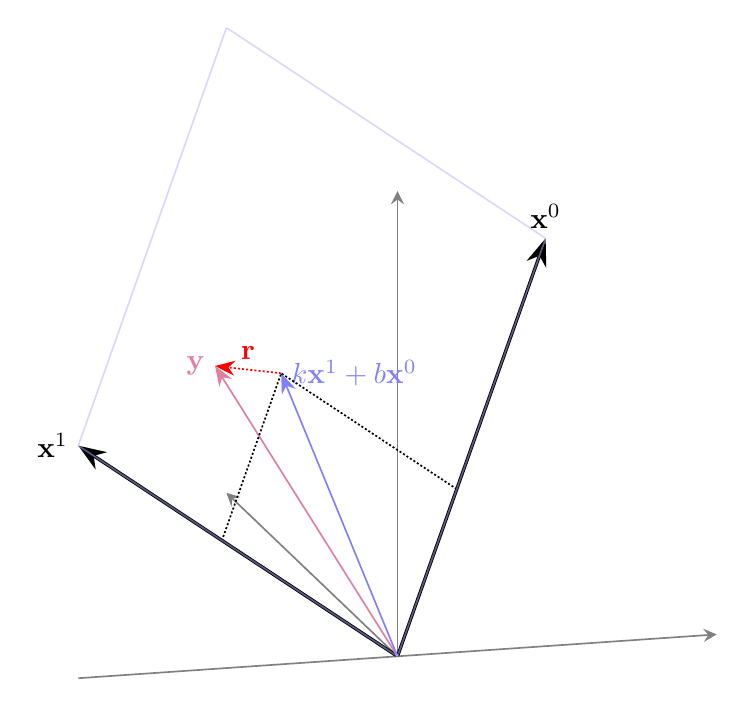
\begin{tikzpicture}[>=Stealth, scale=1.5]
        \begin{axis}[
                view={-15}{20},      % 设置视角 (方位角, 俯仰角)
                axis lines=center,  % 轴从原点开始
                enlargelimits=false,
                ticks=none,         % 取消刻度
                colormap/viridis,
                axis line style={draw=gray},
                % xlabel={$x$},
                % ylabel={$y$},
                % zlabel={$z$}
            ]

            \coordinate (O) at (axis cs:0,0,0);
            \coordinate (Y) at (axis cs:-0.25, 0.6, 0.85);
            \coordinate (A) at (axis cs:-0.15, 0.4, 0.95);

            \addplot3[thick, ->] coordinates {(0,0,0) (1,1,1)} ;
            \node[above, scale=0.7] at (axis cs:1,1,1) {$\bfx^0$};

            \addplot3[thick, ->] coordinates {(0,0,0) (-1,0,1)};
            \node[left, scale=0.7] at (axis cs:-1,0,1) {$\bfx^1$};

            \addplot3[thin, purple!50, ->] coordinates {(0,0,0) (-0.25, 0.6, 0.85)};
            \node[left, purple!50, scale=0.7] at (Y) {$\bfy$};

            \addplot3[thin, blue!50, ->] coordinates {(0,0,0) (-0.15, 0.4, 0.95)};
            \node[right, blue!50, scale=0.7] at (A) {$k\bfx^1 + b\bfx^0$};

            \addplot3[red, dash pattern=on 0.5pt off 0.5pt, ->] coordinates {(-0.15,0.4,0.95) (-0.25, 0.6, 0.85)};
            \node[red, above, scale=0.7] at (axis cs:-0.2, 0.5, 0.9) {$\bfr$};

            \addplot3[thin, dash pattern=on 0.5pt off 0.5pt] coordinates {(0.4, 0.4, 0.4) (-0.15, 0.4, 0.95) (-0.55, 0, 0.55)};

            \addplot3[surf, color=blue!30, fill=blue!30, shader=flat, opacity=0.5]
            coordinates {(0,1,2) (1,1,1) (0,0,0) (-1,0,1) (0,1,2)};
        \end{axis}
    \end{tikzpicture}
    \caption{从几何的角度看残差}
\end{figure}

从几何上,$k\bfx^1 + b\bfx^0$ 落在 $\bfx^0$ 与 $\bfx^1$ 确定的平面上,求 $\bfr = \bfy - (k\bfx^1 + b\bfx^0)$ 的最小值实际上就是从点向平面做垂线并求垂线长。平面上的点恰好表示了那些可以精准拟合的数据,而偏离平面的部分则暗示了无论怎么用直线拟合都会有误差。不得不说从几何上看确实清晰很多,事实上也有人从几何角度给出了\uhref{https://www.bilibili.com/video/BV15zPBevERL}{推导},不过掠过这些细节,仅保留一个直观的印象也无大碍。本节的几篇推荐阅读中都用不同的方法解答了如何最小化误差,有详细的推导,因此这里不再赘述。但是我认为如果读者有一些基础的统计知识而且想记住线性回归推导出的结果,那么结论值得一提,不过跳过也无妨。计算出来的结论是这样的:

首先要计算的是样本中心点,对 $b$ 的导数项为 0 推出最优的直线必然经过样本中心点 $(\bar x, \bar y)$,其中
\[
    \bar x = \frac1n \sum_{i=1}^n x_i, \bar y = \frac1n \sum_{i=1}^n y_i
\]

即\textoverset{Mean}{均值}。

看斜率之前先看看\textoverset{Variance}{方差}和\textoverset{Covariance}{协方差},方差\footnote{此注释写给学过数理统计的读者:此处并非\textoverset{Sample Variance}{样本方差},样本方差除以的是 $n-1$}的表达式是
\[
    \text{Var}(\bfx) = \frac1n \sum_{i=1}^n (x_i - \bar x)^2
\]

是不是感觉很熟悉?这不就是自变量相对均值的 MSE 吗?而协方差的表达式是
\[
    \text{Cov}(\bfx, \bfy) = \frac1n \sum_{i=1}^n (x_i - \bar x)(y_i - \bar y)
\]

它把方差中的平方项换成了 $x$ 和 $x$ 的\textoverset{Cross Term}{交叉项},并由此体现出了\textoverset{Correlation}{相关关系}。接下来计算的是斜率 $k$,它的表达式是
\[
    \hat k = \frac{\sum_{i=1}^n (x_i - \bar x)(y_i - \bar y)}{\sum_{i=1}^n (x_i - \bar x)^2}
\]

虽然分子分母都是求和式,看起来有些复杂,但是总结起来其实就是协方差除以自变量的方差,即 $k = \text{Cov}(\bfx, \bfy) / \text{Var}(\bfx)$,如果把协方差看作一种乘法\footnote{此注释写给熟悉线性代数的同学:在\uhref{https://en.wikipedia.org/wiki/Inner_product_space\#Random_variables}{向量空间内积}的意义上这几乎正确},那么 $k = (\bfx\cdot \bfy) / (\bfx\cdot \bfx)$ 看起来确实挺像那么回事的。

这样一来,通过点-斜率式方程就可以得到最优的直线,那么直线拟合就告一段落了。

\begin{tcolorbox}[myrecommendbox, title=推荐阅读, breakable=false]
    \begin{itemize}
        \item 如果你想了解“回归”与“\textoverset{Least Squares}{最小二乘}”的含义:\\
              \textit{用人话讲明白线性回归Linear Regression - 化简可得的文章 - 知乎}\\
              \url{https://zhuanlan.zhihu.com/p/72513104}
        \item 如果你想阅读从求导法到线性代数方法的详尽公式推理:\\
              \textit{非常详细的线性回归原理讲解 - 小白Horace的文章 - 知乎}\\
              \url{https://zhuanlan.zhihu.com/p/488128941}
        \item 如果你想详细了解了线性回归中的术语、求解过程与几何诠释:\\
              \textit{机器学习| 算法笔记-线性回归(Linear Regression) - iamwhatiwant的文章 - 知乎}\\
              \url{https://zhuanlan.zhihu.com/p/139445419}
    \end{itemize}
\end{tcolorbox}

\newpage

\subsection{多项式拟合}

\begin{figure}[H]
    \centering
    \includegraphics[width=0.6\textwidth]{img/polynomial_fitting.png}
    \caption{多项式拟合示意图(图为 3 次拟合)}
    {图源: \uhref{https://www.geeksforgeeks.org/numpys-polyfit-function-a-comprehensive-guide/}{GeeksforGeeks}}
    \label{fig:polynomial_fitting}
\end{figure}

线性拟合虽然很好,但是如果拿到了明显不线性的一堆数据,那么线性拟合就显得有些力不从心了。不过既然都是拟合,能做一次的那按理来讲也能做多次。\textoverset{Polynomial Fitting}{多项式拟合}就是这样一种思路,只是预测 $\hat y$ 从 $kx+b$ 变成了 $a_0 + a_1 x + \cdots + a_m x^m$\,\footnote{记号说明:虽然习惯上幂次从大到小排列,但是为了下标和幂次的统一性,所以这里选择从常数项到最高次项排列},其中 $m$ 是多项式的次数。而均方误差的表达式甚至几乎不用变,仍然是
\[
    \text{MSE} = \frac1n \sum_{i=1}^n (y_i - \hat y)^2
\]

只不过展开后是一系列的多项式项,待拟合的参数从两个变成了 $m+1$ 个。但是如果观察一下,这个式子仍然是一个(多变量的)二次函数,所以最小化的方法也是一样的。多项式自有多项式的好,能加的项多了,拟合的灵活性也就大了,误差显然会更小。然而与线性拟合相比,它虽然有\textoverset{Analytical Solution}{解析解},但不再像线性拟合一样可以逐项明确说出意义,而是只剩下一堆矩阵运算把这些参数算出来。因此相比于记下公式,形成一个整体上的印象显得尤为重要。

上一小节中,我们从图像看到了这种拟合的几何解释,而多项式拟合也是相似的,还是从 $\bfr$ 的表达式入手
\[
    \bfr = \bfy - (a_0 \bfx^0 + a_1 \bfx^1 + \cdots + a_m \bfx^m)
\]

对比之前的表达式,当 $a_0, a_1, \ldots, a_m$ 变化时,预测得到的结果 $\hat \bfy = a_0 \bfx^0 + a_1 \bfx^1 + \cdots + a_m \bfx^m$ 也会在一个 $m + 1$ 维的空间中变化,正如之前的平面,这个空间也是一个 $m + 1$ 维的子空间。求最小模的 $\bfr$ 又回到了从点到子空间的垂线问题。虽然不得不承认:想象从一个高维的 $n$ 维空间中向 $m+1$ 维的子空间做垂线确实有些困难,但是这多少离我们的几何直觉更近了一些。

系数的意义不那么明确了,但是误差下来了,这是好事吗?也不一定,灵活性的另一面是潜在的\textoverset{Overfitting}{过拟合}。前文中做线性拟合的时候有一个重要的假设是测量得到数据带有一定的误差。拟合的直线滤去了大部分的误差,留下了重要的趋势。但是如果灵活性太高,拟合的多项式会过于贴合数据,甚至把误差也拟合进去了。即使在给定的数据上做到了很小的误差,预测新数据的能力却可能会大打折扣。

拿做题打个比方:使用直线拟合明显不线性的数据是方法错了,只能说是没完全学会。但是用接近数据量的参数来拟合数据,留给它的空间都够把结果“背下来”了,捕捉到了数据的细节,却忽略了数据背后的规律,化成了一种只知道背答案的自我感动。在几道例题上能做到滴水不漏,但是一遇到新题就束手无策。

举个例子,在下面这个数据集上试图拟合,我们在二次函数 $y = 0.25 x^2 - x + 1$ 上添加了标准正态分布的噪声,即实际上 $y = 0.25 x^2 - x + 1 + \mathcal{N}(0, 1)$ \footnote{$\mathcal{N}(0, 1)$:表示一个服从\uhref{https://baike.baidu.com/item/\%E6\%A0\%87\%E5\%87\%86\%E6\%AD\%A3\%E6\%80\%81\%E5\%88\%86\%E5\%B8\%83}{标准正态分布}的变量,均值为 0,方差为 1}。
\newcommand{\drawrawdata}{
    \addplot[
        only marks,
        mark=*,
        color=blue
    ]
    coordinates {
            (0.0, 0.423) (0.1, -0.726) (0.2, 1.96) (0.3, 0.065) (0.4, -0.355) (0.5, 0.45) (0.6, -0.778) (0.7, 0.123) (0.8, 0.531) (0.9, -1.097) (1.0, 1.218) (1.1, -0.018) (1.2, 0.363) (1.3, -2.308) (1.4, -0.688) (1.5, 0.5) (1.6, 1.28) (1.7, -0.052) (1.8, 0.45) (1.9, -0.398) (2.0, 0.207) (2.1, 0.237) (2.2, -1.486) (2.3, 0.244) (2.4, -0.215) (2.5, -0.849) (2.6, 0.395) (2.7, -0.185) (2.8, -0.415) (2.9, -0.477) (3.0, 1.11) (3.1, -0.435) (3.2, 0.833) (3.3, 1.451) (3.4, 0.147) (3.5, 0.139) (3.6, -1.163) (3.7, 3.425) (3.8, -0.117) (3.9, 2.428) (4.0, 1.964) (4.1, 1.613) (4.2, 0.992) (4.3, 0.949) (4.4, 1.707) (4.5, 2.736) (4.6, 0.905) (4.7, 1.117) (4.8, 3.352) (4.9, 3.162) (5.0, 2.226) (5.1, 3.536) (5.2, 1.403) (5.3, 2.448) (5.4, 2.652) (5.5, 3.959) (5.6, 3.705) (5.7, 3.537) (5.8, 3.656) (5.9, 4.784) (6.0, 3.247) (6.1, 4.589) (6.2, 2.857) (6.3, 4.194) (6.4, 4.053) (6.5, 2.536) (6.6, 5.568) (6.7, 5.73) (6.8, 3.667) (6.9, 6.415) (7.0, 4.927) (7.1, 5.545) (7.2, 6.754) (7.3, 6.447) (7.4, 7.352) (7.5, 7.55) (7.6, 8.649) (7.7, 7.145) (7.8, 7.837) (7.9, 7.964) (8.0, 9.074) (8.1, 8.135) (8.2, 10.401) (8.3, 8.005) (8.4, 10.431) (8.5, 10.629) (8.6, 8.624) (8.7, 10.726) (8.8, 13.097) (8.9, 12.136) (9.0, 12.849) (9.1, 10.127) (9.2, 14.107) (9.3, 13.364) (9.4, 14.538) (9.5, 12.474) (9.6, 15.591) (9.7, 13.714) (9.8, 16.952) (9.9, 16.317) (10.0, 16.764)
        };
    \addlegendentry{带噪声数据}
}
\begin{figure}[h]
    \centering
    \begin{tikzpicture}
        \begin{axis}[
                axis lines=middle,
                xlabel={$x$}, ylabel={$y$},
                grid=major,
                legend pos=north west
            ]
            \drawrawdata
            \addplot[
                domain=0:10,
                samples=100,
                color=red,
                thick
            ] {0.25 * x^2 - x + 1};
            \addlegendentry{真实曲线}
        \end{axis}
    \end{tikzpicture}
\end{figure}

那么现在我们来试试用不同次数的多项式拟合这个数据集。不难看出线性拟合的线与数据点还是相差不少,因为它没能提供可以制造数据“弯曲”形状的项,它没能捕捉到数据更加复杂的趋势,这种现象称为\textoverset{Underfitting}{欠拟合}。2 次曲线的效果几乎和真实曲线一样,即使提升到 3 次也没有太明显的改变,它们拟合的效果都还算好。
\begin{figure}[H]
    \centering
    \begin{tikzpicture}
        \begin{axis}[
                axis lines=middle,
                xlabel={$x$}, ylabel={$y$},
                grid=major,
                legend pos=north west
            ]
            \drawrawdata
            \addplot[
                domain=0:10,
                samples=100,
                color=red,
                thick
            ] {0.25 * x^2 - x + 1};
            \addlegendentry{真实曲线}

            \addplot[
                domain=0:10,
                samples=100,
                color=orange,
                thick
            ] {1.5142676761793825 * x -3.3366750145602806};
            \addlegendentry{线性拟合}

            \addplot[
                domain=0:10,
                samples=100,
                color=yellow,
                thick
            ] {0.24383409557403493 * x^2 -0.9240732795609664 * x + 0.6865875624112963};
            \addlegendentry{二次拟合}

            \addplot[
                domain=0:10,
                samples=100,
                color=green,
                thick
            ] {0.012628009463763832 * x^3 + 0.054413953617577414 * x^2 -0.17015585855533788 * x + 0.07400282332411103};
            \addlegendentry{三次拟合}
        \end{axis}
    \end{tikzpicture}
\end{figure}

但是如果继续增加次数呢?先来看看十次的拟合效果。
\begin{figure}[H]
    \centering
    \begin{tikzpicture}
        \begin{axis}[
                axis lines=middle,
                xlabel={$x$}, ylabel={$y$},
                grid=major,
                legend pos=north west
            ]
            \drawrawdata

            \addplot[
                domain=0:10,
                samples=100,
                color=red,
                thick
            ] {0.25 * x^2 - x + 1};
            \addlegendentry{真实曲线}

            \addplot[
                domain=0:10,
                samples=100,
                color=orange,
                thick
            ] {-0.000004129005667 * x^10 + 0.000200033877258 * x^9 - 0.004061827595427 * x^8 + 0.044810202155712 * x^7 - 0.291097682876070 * x^6 + 1.129425113256322 * x^5 - 2.542208192992861 * x^4 + 3.091776048493755 * x^3 - 1.584353162512058 * x^2 - 0.267618886184698 * x + 0.362912675589959};
            \addlegendentry{十次拟合}
        \end{axis}
    \end{tikzpicture}
\end{figure}

你可能会想,虽然是稍微歪了一点,不过这看起来还行吧。但是如果你把 $x$ 的范围稍微扩大一点,你就会发现势头完全不对了。
\begin{figure}[H]
    \centering
    \begin{tikzpicture}
        \begin{axis}[
                axis lines=middle,
                xlabel={$x$}, ylabel={$y$},
                grid=major,
                legend pos=south east
            ]
            \drawrawdata

            \addplot[
                domain=-1.5:11.5,
                samples=100,
                color=red,
                thick
            ] {0.25 * x^2 - x + 1};
            \addlegendentry{真实曲线}

            \addplot[
                domain=-1.5: 11.5,
                samples=100,
                color=orange,
                thick
            ] {(((((((((-0.000004129005667 * x + 0.000200033877258) * x - 0.004061827595427) * x + 0.044810202155712) * x - 0.291097682876070) * x + 1.129425113256322) * x - 2.542208192992861) * x + 3.091776048493755) * x - 1.584353162512058) * x - 0.267618886184698) * x + 0.362912675589959};
            \addlegendentry{十次拟合}
        \end{axis}
    \end{tikzpicture}
\end{figure}

一旦离开了拟合的区域,十次拟合的曲线就直勾勾地弯向无穷远,这是因为它把噪声也拟合进去了,从而给出了\textoverset{Generalization}{泛化性}\footnote{泛化性:预测原有数据集以外点的能力}极差的结果。这就是过拟合的危害。因为参数量与样本点数量并没有非常显著的差别(10 个参数,100 个样本点),所以从去噪声的角度看,结果过拟合并不奇怪——过滤掉噪声需要更多的数据。

当然解决办法并不是没有,要解决问题先要找到问题的根源。既然得到的函数行为不符合预期,那么很自然地我们会想问,这个函数的系数怎么样呢?在上面这个具体的例子中,函数的表达式是
\[
    \begin{aligned}
        \hat y & = -0.000004129005667 x^{10} + 0.000200033877258 x^9 - 0.004061827595427 x^8   \\
               & \quad + 0.044810202155712 x^7 - 0.291097682876070 x^6 + 1.129425113256322 x^5 \\
               & \quad - 2.542208192992861 x^4 + 3.091776048493755 x^3 - 1.584353162512058 x^2 \\
               & \quad - 0.267618886184698 x + 0.362912675589959
    \end{aligned}
\]

简单估算一下就会发现,例如 3, 4 次项的系数都在个位数级别,再乘以 $x$ 的 3 次方、4 次方数值就会变得很大。10 次方项的系数看起来只有 $4.1\times 10^{-6}$,但是乘上 $\bfx$ 中最大值的 10 次方,也就是 $10^{10}$ 后,这个数值同样会飙升到上万的级别。一堆上万级别的数加在一起,倒不如说顶着舍入误差\footnote{舍入误差:就像手动计算时保留几位小数一样,计算机计算的并不是“实数”,而是具有一定精度的浮点数,同样也有误差。例如对于 32-bit 的浮点数,只能精确到 7 个十进制位,这意味着从万位向后数到第 7 位,从百分位就可能已经不准确,在此之后的数位就不太可靠了。}还能够回归到原来的数据集上已经是奇迹了。也就只有 MSE 可以限制一下它在数据集内的行为,出了预定义的范围,这个高次函数大概就放飞自我了。

不过如果一定要用高次函数,补救的办法也不是没有。既然这些系数导致了很大的数值,那限制一下这些数值就好了,这就是\textoverset{Regularization}{正则化}的思路。我们在待优化的函数上加上一个\textoverset{Penalty Term}{惩罚项},同样地使用平方求和的形式,只不过这次是对系数进行惩罚,为了让系数尽量小,即尽量贴近于 $0$,自然想到把它们乘以权重后的平方也加起来,优化的目标\footnote{Loss:损失,与前文单纯使用 MSE 时相同,我们希望让它尽可能小,它的每一项包含了我们对拟合结果的一个美好“祝愿”,MSE 项希望它误差减小,正则化项希望它系数正常。}变成了
\[
    \text{Loss} = \text{MSE} + \underset{\text{正则化项}}{\underbrace{\sum_{i=1}^{10} (\mu_i a_i)^2}}
\]

可调参数 $\mu_i$ 表明我们希望在多大程度上抑制每个系数,在这个例子中不同次项的权重可能并不相同,不过在后续拟合的许多例子中这个会使用统一的权重,即所有的 $\mu_i$ 均为相同的定值 $\mu$,式子从而变为了一个常数 $\lambda = \mu^2$ 倍的平方和。为每一项设置分立的系数是为了解决一个致命的问题:不同系数对最终结果的影响可能不同。例如在 $x=10$ 这一点上,$x^{10}$ 项的系数对结果的影响远远大于 $x$ 项的系数,即使是 $4.1\times 10^{-6}$ 这样微小的 $10$ 次项系数也会导致非常大的数值。平方后这一系数变得十分微小,原本用于约束系数大小的正则化项对它的影响更是微乎其微。

不过即使我们使用了相同的系数 $\lambda$,也仍然有一些技巧可以帮我们把高次项压下去。我们发现一路下来导致问题的根源都是 $x$ 的高次项即使在系数很小时也会导致数值爆炸。但是如果把 $x$ 放到 $[-1, 1]$ 的闭区间内呢?这样即使是 $x^{10}$ 项,$x$ 的 10 次方也不会超过 $1$,系数再怎么大,至少在小范围内也不会导致数值爆炸,这样一来正则化项才能发挥其约束作用。

操作上只需要把 $[0, 10]$ 范围内的 $x$ 线性地映射到 $[-1, 1]$ 范围内。这很简单,令 $z = 0.2 x - 1$ 再对 $y$ 用 $z$ 的多项式拟合,这种操作称作\textoverset{Normalization}{归一化}\footnote{归一化:调整数据到某个给定的范围内,使数据在不同场景下更加可比、更加数值稳定。前文计算误差时取平均实际上也是一种归一化。}。

事实上只需要一个很小的 $\lambda$ 就可以在一定程度上抑制高次项的系数,这里我们取 $\lambda = 0.01$,优化的目标变为了
\[
    \text{Loss} = \text{MSE} + 0.01 \sum_{i=1}^{10} a_i^2
\]

这时拟合出来的图像是这样的:

\begin{figure}[H]
    \centering
    \begin{tikzpicture}
        \begin{axis}[
                axis lines=middle,
                xlabel={$z$}, ylabel={$y$},
                grid=major,
                legend pos=north west
            ]

            \addplot[
                only marks,
                mark=*,
                color=blue
            ] coordinates {
                    (-1.0, 0.423) (-0.98, -0.726) (-0.96, 1.96) (-0.94, 0.065) (-0.92, -0.355) (-0.9, 0.45) (-0.88, -0.778) (-0.86, 0.123) (-0.84, 0.531) (-0.82, -1.097) (-0.8, 1.218) (-0.78, -0.018) (-0.76, 0.363) (-0.74, -2.308) (-0.72, -0.688) (-0.7, 0.5) (-0.68, 1.28) (-0.66, -0.052) (-0.64, 0.45) (-0.62, -0.398) (-0.6, 0.207) (-0.58, 0.237) (-0.56, -1.486) (-0.54, 0.244) (-0.52, -0.215) (-0.5, -0.849) (-0.48, 0.395) (-0.46, -0.185) (-0.44, -0.415) (-0.42, -0.477) (-0.4, 1.11) (-0.38, -0.435) (-0.36, 0.833) (-0.34, 1.451) (-0.32, 0.147) (-0.3, 0.139) (-0.28, -1.163) (-0.26, 3.425) (-0.24, -0.117) (-0.22, 2.428) (-0.2, 1.964) (-0.18, 1.613) (-0.16, 0.992) (-0.14, 0.949) (-0.12, 1.707) (-0.1, 2.736) (-0.08, 0.905) (-0.06, 1.117) (-0.04, 3.352) (-0.02, 3.162) (0.0, 2.226) (0.02, 3.536) (0.04, 1.403) (0.06, 2.448) (0.08, 2.652) (0.1, 3.959) (0.12, 3.705) (0.14, 3.537) (0.16, 3.656) (0.18, 4.784) (0.2, 3.247) (0.22, 4.589) (0.24, 2.857) (0.26, 4.194) (0.28, 4.053) (0.3, 2.536) (0.32, 5.568) (0.34, 5.73) (0.36, 3.667) (0.38, 6.415) (0.4, 4.927) (0.42, 5.545) (0.44, 6.754) (0.46, 6.447) (0.48, 7.352) (0.5, 7.55) (0.52, 8.649) (0.54, 7.145) (0.56, 7.837) (0.58, 7.964) (0.6, 9.074) (0.62, 8.135) (0.64, 10.401) (0.66, 8.005) (0.68, 10.431) (0.7, 10.629) (0.72, 8.624) (0.74, 10.726) (0.76, 13.097) (0.78, 12.136) (0.8, 12.849) (0.82, 10.127) (0.84, 14.107) (0.86, 13.364) (0.88, 14.538) (0.9, 12.474) (0.92, 15.591) (0.94, 13.714) (0.96, 16.952) (0.98, 16.317) (1.0, 16.764)
                };
            \addlegendentry{带噪声数据}

            \addplot[
                domain=-1.4: 1.4,
                samples=100,
                color=red,
                thick
            ] {0.25 * ((x+1)*5)^2 - (x+1)*5 + 1};
            \addlegendentry{真实曲线}

            \addplot[
                domain=-1.4:1.4,
                samples=100,
                color=orange,
                thick
            ] {0.056914714852145956 * x^10
                -0.16883868373880576 * x^9
                +0.2748227691835253 * x^8
                +0.02818103309527224 * x^7
                +0.8506420254328089 * x^6
                +0.5250028027489858 * x^5
                +1.8635063516688952 * x^4
                +1.8797071938317609 * x^3
                +3.414068726324771 * x^2
                +6.0490130644654645 * x^1
                +2.5048936484111635};
            \addlegendentry{十次拟合}
        \end{axis}
    \end{tikzpicture}
\end{figure}
\let\drawrawdata\relax

虽然图中拟合曲线与真值在数据集外确实仍然有显著的差距,但经过自变量归一化和参数正则化项的加入,拟合的曲线至少把数据的大体趋势成功地延伸到了数据集的一个邻域内,不至于像原本的那样惨不忍睹。

不过在实际应用中,几乎不会用到 5 次以上的多项式拟合。仍然是因为容易过拟合:就以 $[-1, 1]$ 上的函数为例,$x^5$ 与 $x^7$ 的图像几乎是一样的,它们最大的差值仅为 0.12,这意味着如果允许的高次项太多,一点点微小的噪声就能让轻易地把五次项的系数“分给”七次项,或者反之。这导致拟合的数值稳定性很差,因此显然不太可靠。从这种影响的角度看,高次多项式拟合本身就有\textoverset{Singularity}{奇异性},解并不稳定(这种对微小噪声敏感的问题常称为\textoverset{Ill-posed Problem}{病态问题})。因此比正则化或者归一化更重要的是,我们应该意识到高次函数并不是万能的。当你觉得需要用到很高次的函数才能成功拟合时,不如先想想,多项式的假设真的合适吗?

我们注意到一个重要的事实:虽然拟合的参数在变化,但是拟合前仍然需要人为地设定多项式的次数,正则项(如果有的话)权重也需要人为设定。这些\textoverset{Prior}{先验}的\footnote{先验:在观测到数据之前,我们已经了解了一些数据特征。}参数通常称为\textoverset{Hyperparameter}{超参数}。如何用模型拟合固然是重要的问题,但是模型的结构,包括如何选取适当的超参数也有学问。因为它们通常不是直接从数据中学习的,而需要人为设定。\uhref{https://www.zhihu.com/question/625846838/answer/3251736042}{有道是}“学而不思则欠拟合,思而不学则过拟合”。参数太少就会像那直线拟合曲线一样,必然导致拟合的精度不足。参数太多则会受到太多的噪声干扰,像是拿高次函数拟合低次函数一样因为一点噪声导致函数行为夸张,在预定义的数据集外两眼一抹黑。只有在一定程度上了解问题的本质,才能选出合适的拟合模型。

\begin{tcolorbox}[myrecommendbox, title=推荐阅读, breakable=false]
    \begin{itemize}
        \item 如果你想看更多关于多项式拟合的实战,可以阅读:\\
              \textit{多项式拟合的介绍与例子 - 姓甚名谁的文章 - 知乎}\\
              \url{https://zhuanlan.zhihu.com/p/366870301}
        \item 如果你曾经想过拿问卷调查来做拟合,可以看看:\\
              \textit{理科生觉得哪些知识不知道是文科生的遗憾? - 一只小猫咪的回答 - 知乎}\\
              \url{https://www.zhihu.com/question/270455074/answer/2374983755}
        \item 这个比喻很好,同一问题下的其它回答也很有趣:\\
              \textit{人的大脑会不会出现“过拟合”病? - 莲梅莉usamimeri的回答 - 知乎}\\
              \url{https://www.zhihu.com/question/625846838/answer/3250463511}
    \end{itemize}
\end{tcolorbox}

\newpage

\subsection{高维的线性拟合}

\begin{figure}[H]
    \centering
    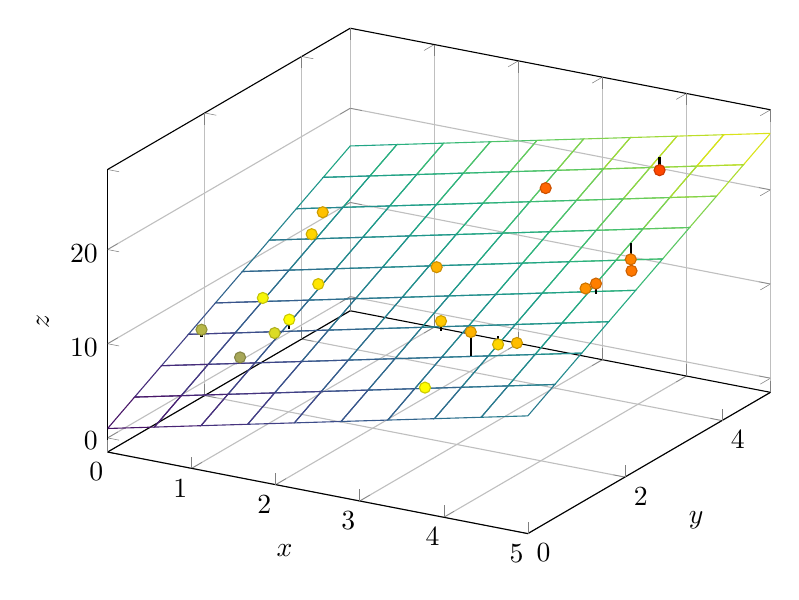
\begin{tikzpicture}
        \begin{axis}[
                view={30}{30}, % 3D视角
                xlabel={$x$}, % x轴标签
                ylabel={$y$}, % y轴标签
                zlabel={$z$}, % z轴标签
                grid=both, % 显示网格
                width=10cm, % 图形宽度
                height=8cm, % 图形高度
            ]

            % 绘制三维回归曲面
            \addplot3[
                mesh,
                domain=0:5,
                y domain=0:5,
                samples=10, % 控制采样的精细度
                colormap/viridis % 曲面的颜色映射
            ]
            {2*x + 3*y + 1}; % 这是回归方程 z = 2x + 3y + 1

            % 绘制数据点
            \addplot3[
                only marks,
                scatter,
                mark=*, % 点的形状
                red
            ] coordinates {
                    (3.795, 1.474, 12.073)
                    (1.06, 1.606, 8.15)
                    (4.727, 2.609, 18.101)
                    (3.045, 1.597, 12.882)
                    (2.382, 2.655, 14.288)
                    (2.869, 4.058, 19.319)
                    (4.354, 2.308, 16.486)
                    (4.556, 2.173, 17.759)
                    (3.427, 0.605, 9.461)
                    (0.542, 2.26, 9.017)
                    (0.187, 1.612, 6.976)
                    (1.109, 2.421, 10.991)
                    (3.897, 4.625, 21.301)
                    (0.437, 3.448, 12.044)
                    (3.68, 1.11, 14.286)
                    (0.387, 3.763, 13.343)
                    (1.171, 1.715, 9.446)
                    (0.881, 1.204, 6.461)
                    (4.165, 1.221, 13.633)
                    (4.448, 3.077, 17.432)
                };

            % 绘制数据点到平面竖直方向的连线
            \draw[black, thick] (axis cs:3.795,1.474,12.073) -- (axis cs:3.795,1.474,13.012);
            \draw[black, thick] (axis cs:1.06,1.606,8.15) -- (axis cs:1.06,1.606,7.938);
            \draw[black, thick] (axis cs:4.727,2.609,18.101) -- (axis cs:4.727,2.609,18.281);
            \draw[black, thick] (axis cs:3.045,1.597,12.882) -- (axis cs:3.045,1.597,11.881);
            \draw[black, thick] (axis cs:2.382,2.655,14.288) -- (axis cs:2.382,2.655,13.729);
            \draw[black, thick] (axis cs:2.869,4.058,19.319) -- (axis cs:2.869,4.058,18.912);
            \draw[black, thick] (axis cs:4.354,2.308,16.486) -- (axis cs:4.354,2.308,16.632);
            \draw[black, thick] (axis cs:4.556,2.173,17.759) -- (axis cs:4.556,2.173,16.631);
            \draw[black, thick] (axis cs:3.427,0.605,9.461) -- (axis cs:3.427,0.605,9.669);
            \draw[black, thick] (axis cs:0.542,2.26,9.017) -- (axis cs:0.542,2.26,8.864);
            \draw[black, thick] (axis cs:0.187,1.612,6.976) -- (axis cs:0.187,1.612,6.21);
            \draw[black, thick] (axis cs:1.109,2.421,10.991) -- (axis cs:1.109,2.421,10.481);
            \draw[black, thick] (axis cs:3.897,4.625,21.301) -- (axis cs:3.897,4.625,22.669);
            \draw[black, thick] (axis cs:0.437,3.448,12.044) -- (axis cs:0.437,3.448,12.218);
            \draw[black, thick] (axis cs:3.68,1.11,14.286) -- (axis cs:3.68,1.11,11.69);
            \draw[black, thick] (axis cs:0.387,3.763,13.343) -- (axis cs:0.387,3.763,13.063);
            \draw[black, thick] (axis cs:1.171,1.715,9.446) -- (axis cs:1.171,1.715,8.487);
            \draw[black, thick] (axis cs:0.881,1.204,6.461) -- (axis cs:0.881,1.204,6.374);
            \draw[black, thick] (axis cs:4.165,1.221,13.633) -- (axis cs:4.165,1.221,12.993);
            \draw[black, thick] (axis cs:4.448,3.077,17.432) -- (axis cs:4.448,3.077,19.127);
        \end{axis}
    \end{tikzpicture}
    \caption{高维线性拟合示例}
\end{figure}

第一节我们介绍了“简单线性回归”,即只有一个自变量的线性回归。但是在实际问题中,自变量往往不止一个,这时一元的线性回归就需要改成\textoverset{Multiple Linear Regression}{多元线性回归}。不过按照我的习惯,文中仍然称为“拟合”。

现实世界中的数据往往是多维的,就以估计体重为例,不难发现年龄和身高就是两个可能相关的变量。如果我们想用一个模型来描述这种相关性的话,最简单的就是线性模型了,与之前的 $\hat y=k x+b$ 类似,自然想到用这样的函数\footnote{记号说明:这里使用字母 $w$ 表示\textoverset{weight}{权重},$b$ 表示\textoverset{bias}{偏置},即常数项,$d$ 表示的是空间的\textoverset{dimension}{维度}。}去拟合数据:
\[
    \hat y = w_1 x_1 + w_2 x_2 + \cdots + w_d x_d + b
\]

同样地,优化的目标仍然是最小化均方误差,即对 $n$ 个数据点令
\[
    \text{MSE} = \frac{1}{n} \sum_{i=1}^{n} (y_i - \hat y_i)^2
\]

通过最小化误差得到 $w = [w_1, w_2, \cdots, w_d]$ 和 $b$ 的值。这个过程与一元线性回归的过程是类似的,只不过自变量是一维时,可以在平面上直接画出拟合的直线,二维时可以在空间中画出平面,但是当维数增加到三维及以上时,拟合所用的线性函数就变为\textoverset{Hyperplane}{超平面}了,我们无法直观地看到这个超平面,但是可以猜测,它的原理差不多。

话不多说,先看看效果。这里以美国人类学家 Richard McElreath 搜集到的一个年龄、身高与体重\uhref{https://github.com/rmcelreath/rethinking/blob/master/data/Howell1.csv}{数据集}为例,它的分布与拟合出来的平面是这样的:
\def\howelldata{
    (63.0, 151.765, 47.8256065) (63.0, 139.7, 36.4858065) (65.0, 136.525, 31.864838) (41.0, 156.845, 53.0419145) (51.0, 145.415, 41.276872) (35.0, 163.83, 62.992589) (32.0, 149.225, 38.2434755) (27.0, 168.91, 55.4799715) (19.0, 147.955, 34.869885) (54.0, 165.1, 54.487739) (47.0, 154.305, 49.89512) (66.0, 151.13, 41.220173) (73.0, 144.78, 36.0322145) (20.0, 149.9, 47.7) (65.3, 150.495, 33.849303) (36.0, 163.195, 48.5626935) (44.0, 157.48, 42.3258035) (31.0, 143.9418, 38.3568735) (12.0, 121.92, 19.617854) (8.0, 105.41, 13.947954) (6.5, 86.36, 10.489315) (39.0, 161.29, 48.987936) (29.0, 156.21, 42.7226965) (13.0, 129.54, 23.586784) (7.0, 109.22, 15.989118) (56.0, 146.4, 35.493574) (45.0, 148.59, 37.9032815) (19.0, 147.32, 35.4652245) (17.0, 137.16, 27.328918) (16.0, 125.73, 22.6796) (11.0, 114.3, 17.860185) (29.0, 147.955, 40.312989) (30.0, 161.925, 55.111428) (24.0, 146.05, 37.5063885) (35.0, 146.05, 38.498621) (33.0, 152.7048, 46.606578) (27.0, 142.875, 38.838815) (32.0, 142.875, 35.5786225) (36.0, 147.955, 47.400364) (24.0, 160.655, 47.8823055) (30.0, 151.765, 49.4131785) (24.0, 162.8648, 49.384829) (52.0, 171.45, 56.5572525) (42.0, 147.32, 39.12231) (19.0, 147.955, 49.89512) (17.0, 144.78, 28.803092) (8.0, 121.92, 20.41164) (12.0, 128.905, 23.359988) (5.0, 97.79, 13.267566) (55.0, 154.305, 41.2485225) (43.0, 143.51, 38.55532) (20.0, 146.7, 42.4) (18.0, 157.48, 44.6504625) (13.0, 127.0, 22.0105518) (9.0, 110.49, 15.422128) (5.0, 97.79, 12.757275) (42.0, 165.735, 58.5984165) (44.0, 152.4, 46.719976) (60.0, 141.605, 44.22522) (20.0, 158.8, 50.9) (37.0, 155.575, 54.317642) (50.0, 164.465, 45.8978405) (50.0, 151.765, 48.024053) (31.0, 161.29, 52.219779) (25.0, 154.305, 47.62716) (23.0, 145.415, 45.642695) (52.0, 145.415, 42.410852) (79.3, 152.4, 36.4858065) (35.0, 163.83, 55.9335635) (27.0, 144.145, 37.194544) (13.0, 129.54, 24.550667) (14.0, 129.54, 25.627948) (38.0, 153.67, 48.307548) (39.0, 142.875, 37.3362915) (12.0, 146.05, 29.596878) (30.0, 167.005, 47.173568) (24.0, 158.4198, 47.286966) (0.599999999999909, 91.44, 12.927372) (51.0, 165.735, 57.549485) (46.0, 149.86, 37.931631) (17.0, 147.955, 41.900561) (12.0, 137.795, 27.5840635) (22.0, 154.94, 47.2019175) (29.0, 160.9598, 43.204638) (38.0, 161.925, 50.2636635) (30.0, 147.955, 39.3774555) (6.0, 113.665, 17.463292) (45.0, 159.385, 50.689) (47.0, 148.59, 39.4341545) (79.0, 136.525, 36.28736) (45.0, 158.115, 46.266384) (54.0, 144.78, 42.2691045) (31.0, 156.845, 47.62716) (23.0, 179.07, 55.7067675) (9.0, 118.745, 18.824068) (41.0, 170.18, 48.5626935) (23.0, 146.05, 42.807745) (36.0, 147.32, 35.0683315) (5.0, 113.03, 17.8885345) (30.0, 162.56, 56.755699) (12.0, 133.985, 27.442316) (34.0, 152.4, 51.255896) (44.0, 160.02, 47.230267) (43.0, 149.86, 40.936678) (73.3, 142.875, 32.715323) (38.0, 167.005, 57.0675435) (43.0, 159.385, 42.977842) (33.0, 154.94, 39.9444455) (16.0, 148.59, 32.4601775) (11.0, 111.125, 17.123098) (6.0, 111.76, 16.499409) (35.0, 162.56, 45.9545395) (29.0, 152.4, 41.106775) (12.0, 124.46, 18.257078) (9.0, 111.76, 15.081934) (7.59999999999991, 86.36, 11.4815475) (58.0, 170.18, 47.5988105) (53.0, 146.05, 37.5063885) (51.0, 159.385, 45.019006) (48.0, 151.13, 42.2691045) (29.0, 160.655, 54.8562825) (41.0, 169.545, 53.523856) (81.75, 158.75, 52.1914295) (1.0, 74.295, 9.752228) (35.0, 149.86, 42.410852) (46.0, 153.035, 49.5832755) (5.0, 96.52, 13.097469) (29.0, 161.925, 41.730464) (42.0, 162.56, 56.018612) (27.0, 149.225, 42.1557065) (8.0, 116.84, 19.391058) (6.0, 100.076, 15.081934) (22.0, 163.195, 53.0986135) (43.0, 161.925, 50.235314) (53.0, 145.415, 42.52425) (43.0, 163.195, 49.101334) (41.0, 151.13, 38.498621) (50.0, 150.495, 49.8100715) (15.0, 141.605, 29.313383) (33.0, 170.815, 59.760746) (3.0, 91.44, 11.7083435) (62.0, 157.48, 47.9390045) (49.0, 152.4, 39.292407) (17.0, 149.225, 38.1300775) (12.0, 129.54, 21.999212) (22.0, 147.32, 36.8826995) (29.0, 145.415, 42.127357) (8.0, 121.92, 19.787951) (5.0, 113.665, 16.782904) (33.0, 157.48, 44.565414) (34.0, 154.305, 47.853956) (12.0, 120.65, 21.1770765) (7.0, 115.6, 18.9) (42.0, 167.005, 55.1964765) (40.0, 142.875, 32.998818) (27.0, 152.4, 40.879979) (3.0, 96.52, 13.267566) (25.0, 160.0, 51.2) (29.0, 159.385, 49.044635) (45.0, 149.86, 53.4388075) (26.0, 160.655, 54.090846) (45.0, 160.655, 55.3665735) (45.0, 149.225, 42.240755) (11.0, 125.095, 22.3677555) (85.5999999999999, 140.97, 40.936678) (26.0, 154.94, 49.6966735) (24.0, 141.605, 44.338618) (57.0, 160.02, 45.9545395) (22.0, 150.1648, 41.95726) (24.0, 155.575, 51.482692) (6.0, 103.505, 12.757275) (4.0, 94.615, 13.0124205) (21.0, 156.21, 44.111822) (79.0, 153.035, 32.205032) (50.0, 167.005, 56.755699) (40.0, 149.86, 52.673371) (64.0, 147.955, 36.4858065) (32.0, 159.385, 48.8461885) (38.7, 161.925, 56.9541455) (26.0, 155.575, 42.0990075) (63.0, 159.385, 50.178615) (62.0, 146.685, 46.549879) (22.0, 172.72, 61.80191) (41.0, 166.37, 48.987936) (19.0, 141.605, 31.524644) (17.0, 142.875, 32.205032) (14.0, 133.35, 23.756881) (9.0, 127.635, 24.4089195) (7.0, 119.38, 21.5172705) (74.0, 151.765, 35.2951275) (41.0, 156.845, 45.642695) (33.0, 148.59, 43.885026) (53.0, 157.48, 45.5576465) (18.0, 149.86, 39.008912) (37.0, 147.955, 41.163474) (6.0, 102.235, 13.1258185) (61.0, 153.035, 45.245802) (44.0, 160.655, 53.637254) (35.0, 149.225, 52.3048275) (7.0, 114.3, 18.3421265) (4.0, 100.965, 13.7495075) (23.0, 138.43, 39.0939605) (4.0, 91.44, 12.530479) (55.0, 162.56, 45.699394) (53.0, 149.225, 40.3980375) (59.0, 158.75, 51.482692) (57.0, 149.86, 38.668718) (35.0, 158.115, 39.235708) (29.0, 156.21, 44.338618) (62.0, 148.59, 39.519203) (18.0, 143.51, 31.071052) (51.0, 154.305, 46.776675) (14.0, 131.445, 22.509503) (19.0, 157.48, 40.6248335) (42.0, 157.48, 50.178615) (25.0, 154.305, 41.276872) (6.0, 107.95, 17.57669) (41.0, 168.275, 54.6) (37.0, 145.415, 44.9906565) (16.0, 147.955, 44.735511) (5.0, 100.965, 14.401546) (9.0, 113.03, 19.050864) (82.0, 149.225, 35.8054185) (28.0, 154.94, 45.2174525) (50.0, 162.56, 48.1091015) (43.0, 156.845, 45.6710445) (8.0, 123.19, 20.808533) (31.0, 161.0106, 48.420946) (67.0, 144.78, 41.1918235) (39.0, 143.51, 38.4135725) (18.0, 149.225, 42.127357) (11.0, 110.49, 17.6617385) (48.0, 149.86, 38.2434755) (30.0, 165.735, 48.3358975) (64.0, 144.145, 38.9238635) (72.0, 157.48, 40.029494) (68.0, 154.305, 50.2069645) (44.0, 163.83, 54.2892925) (43.0, 156.21, 45.6) (16.0, 153.67, 40.766581) (13.0, 134.62, 27.1304715) (34.0, 144.145, 39.4341545) (10.0, 114.3, 20.4966885) (62.0, 162.56, 43.204638) (44.0, 146.05, 31.864838) (11.0, 120.65, 20.8935815) (31.0, 154.94, 45.4442485) (29.0, 144.78, 38.045029) (8.0, 106.68, 15.989118) (62.0, 146.685, 36.0889135) (67.0, 152.4, 40.879979) (57.0, 163.83, 47.910655) (32.0, 165.735, 47.7122085) (24.0, 156.21, 46.379782) (77.0, 152.4, 41.163474) (62.0, 140.335, 36.5992045) (17.0, 158.115, 43.09124) (67.0, 163.195, 48.137451) (70.0, 151.13, 36.7126025) (37.0, 171.1198, 56.5572525) (58.0, 149.86, 38.6970675) (35.0, 163.83, 47.4854125) (30.0, 141.605, 36.2023115) (5.0, 93.98, 14.288148) (26.0, 149.225, 41.276872) (5.0, 105.41, 15.2236815) (21.0, 146.05, 44.7638605) (41.0, 161.29, 50.4337605) (46.0, 162.56, 55.281525) (49.0, 145.415, 37.931631) (15.0, 145.415, 35.493574) (28.0, 170.815, 58.456669) (12.0, 127.0, 21.488921) (83.0, 159.385, 44.4236665) (54.0, 159.4, 44.4) (54.0, 153.67, 44.565414) (68.0, 160.02, 44.622113) (68.0, 150.495, 40.483086) (56.0, 149.225, 44.0834725) (15.0, 127.0, 24.4089195) (57.0, 142.875, 34.416293) (22.0, 142.113, 32.772022) (40.0, 147.32, 35.947166) (19.0, 162.56, 49.5549) (41.0, 164.465, 53.183662) (75.9000000000001, 160.02, 37.081146) (73.9000000000001, 153.67, 40.5114355) (49.0, 167.005, 50.6038575) (26.0, 151.13, 43.9700745) (17.0, 147.955, 33.792604) (13.0, 125.3998, 21.375523) (8.0, 111.125, 16.669506) (88.0, 153.035, 49.89) (68.0, 139.065, 33.5941575) (33.0, 152.4, 43.8566765) (26.0, 154.94, 48.137451) (56.0, 147.955, 42.751046) (16.0, 143.51, 34.8415355) (13.0, 117.983, 24.097075) (34.0, 144.145, 33.906002) (5.0, 92.71, 12.076887) (17.0, 147.955, 41.276872) (74.0, 155.575, 39.7176495) (69.0, 150.495, 35.947166) (50.0, 155.575, 50.915702) (44.0, 154.305, 45.756093) (15.0, 130.6068, 25.2594045) (5.0, 101.6, 15.3370795) (18.0, 157.48, 49.214732) (41.0, 168.91, 58.8252125) (27.0, 150.495, 43.4597835) (8.90000000000009, 111.76, 17.8318355) (38.0, 160.02, 51.9646335) (57.0, 167.64, 50.688906) (64.5, 144.145, 34.246196) (42.0, 145.415, 39.3774555) (24.0, 160.02, 59.5622995) (16.0, 147.32, 40.312989) (71.0, 164.465, 52.16308) (49.5, 153.035, 39.972795) (33.0, 149.225, 43.941725) (28.0, 160.02, 54.601137) (47.0, 149.225, 45.075705) (3.0, 85.09, 11.453198) (1.0, 84.455, 11.7650425) (1.0, 59.6138, 5.896696) (3.0, 92.71, 12.1052365) (6.0, 111.125, 18.313777) (5.0, 90.805, 11.3681495) (27.0, 153.67, 41.333571) (5.0, 99.695, 16.2442635) (1.0, 62.484, 6.80388) (2.0, 81.915, 11.8784405) (2.0, 96.52, 14.968536) (1.0, 80.01, 9.865626) (55.0, 150.495, 41.900561) (83.4000000000001, 151.765, 42.524) (12.0, 140.6398, 28.859791) (2.0, 88.265, 12.7856245) (63.0, 158.115, 43.147939) (52.0, 149.225, 40.82328) (49.0, 151.765, 42.864444) (31.0, 154.94, 46.209685) (9.0, 123.825, 20.581737) (6.0, 104.14, 15.87572) (35.0, 161.29, 47.853956) (35.0, 148.59, 42.52425) (7.0, 97.155, 17.066399) (5.0, 93.345, 13.1825175) (24.0, 160.655, 48.5059945) (41.0, 157.48, 45.869491) (32.0, 167.005, 52.900167) (43.0, 157.48, 47.570461) (6.0, 91.44, 12.927372) (1.0, 60.452, 5.6699) (15.0, 137.16, 28.91649) (63.0, 152.4, 43.544832) (21.0, 152.4, 43.431434) (1.0, 81.28, 11.509897) (2.0, 109.22, 11.7083435) (1.0, 71.12, 7.540967) (3.0, 89.2048, 12.700576) (1.0, 67.31, 7.200773) (1.0, 85.09, 12.360382) (1.0, 69.85, 7.7961125) (55.0, 161.925, 53.2120115) (38.0, 152.4, 44.678812) (3.0, 88.9, 12.5588285) (3.0, 90.17, 12.700576) (1.0, 71.755, 7.37087) (1.0, 83.82, 9.2135875) (28.0, 159.385, 47.2019175) (16.0, 142.24, 28.632995) (36.0, 142.24, 31.6663915) (38.0, 168.91, 56.4438545) (12.0, 123.19, 20.014747) (1.0, 74.93, 8.50485) (1.0, 74.295, 8.3064035) (3.0, 90.805, 11.623295) (48.0, 160.02, 55.791816) (1.0, 67.945, 7.9662095) (15.0, 135.89, 27.21552) (45.0, 158.115, 47.4854125) (3.0, 85.09, 10.8011595) (3.0, 93.345, 14.004653) (38.0, 152.4, 45.1607535) (21.0, 155.575, 45.529297) (50.0, 154.305, 48.874538) (41.0, 156.845, 46.5782285) (13.0, 120.015, 20.128145) (8.0, 114.3, 18.14368) (3.0, 83.82, 10.9145575) (30.0, 156.21, 43.885026) (12.0, 137.16, 27.158821) (7.0, 114.3, 19.050864) (4.0, 93.98, 13.834556) (21.0, 168.275, 56.0469615) (38.0, 147.955, 40.086193) (15.0, 139.7, 26.5634815) (19.0, 157.48, 50.802304) (1.0, 76.2, 9.2135875) (1.0, 66.04, 7.5693165) (31.0, 160.7, 46.3) (8.0, 114.3, 19.4194075) (16.0, 146.05, 37.9032815) (21.0, 161.29, 49.3564795) (0.0, 69.85, 7.314171) (13.0, 133.985, 28.1510535) (0.0, 67.945, 7.824462) (50.0, 150.495, 44.111822) (39.0, 163.195, 51.0291) (44.0, 148.59, 40.766581) (36.0, 148.59, 37.5630875) (36.0, 161.925, 51.59609) (18.0, 153.67, 44.8205595) (0.0, 68.58, 8.0229085) (58.0, 151.13, 43.4030845) (58.0, 163.83, 46.719976) (33.0, 153.035, 39.5475525) (21.5, 151.765, 34.7848365) (11.0, 132.08, 22.792998) (26.0, 156.21, 39.292407) (22.0, 140.335, 37.4496895) (28.0, 158.75, 48.6760915) (42.0, 142.875, 35.606972) (2.0, 84.455, 9.3836845) (21.0, 151.9428, 43.714929) (19.0, 161.29, 48.19415) (13.0, 127.9906, 29.8520235) (48.0, 160.9852, 50.972401) (46.0, 144.78, 43.998424) (11.0, 132.08, 28.292801) (8.0, 117.983, 20.354941) (25.0, 160.02, 48.19415) (16.0, 154.94, 39.179009) (51.0, 160.9852, 46.6916265) (25.0, 165.989, 56.415505) (28.0, 157.988, 48.591043) (26.0, 154.94, 48.2224995) (5.0, 97.9932, 13.2959155) (1.0, 64.135, 6.6621325) (54.0, 160.655, 47.4854125) (66.0, 147.32, 35.550273) (20.0, 146.7, 36.6) (25.0, 147.32, 48.9595865) (38.0, 172.9994, 51.255896) (51.0, 158.115, 46.5215295) (48.0, 147.32, 36.967748) (13.0, 124.9934, 25.117657) (6.0, 106.045, 16.272613) (27.0, 165.989, 48.647742) (22.0, 149.86, 38.045029) (1.0, 76.2, 8.50485) (60.0, 161.925, 47.286966) (15.0, 140.0048, 28.3495) (0.0, 66.675, 8.1363065) (0.0, 62.865, 7.200773) (43.0, 163.83, 55.394923) (12.0, 147.955, 32.488527) (27.0, 160.02, 54.204244) (30.0, 154.94, 48.477645) (29.0, 152.4, 43.0628905) (0.0, 62.23, 7.257472) (23.0, 146.05, 34.189497) (30.0, 151.9936, 49.951819) (17.0, 157.48, 41.3052215) (0.0, 55.88, 4.8477645) (0.0, 60.96, 6.23689) (41.0, 151.765, 44.338618) (42.0, 144.78, 33.45241) (7.0, 118.11, 16.896302) (3.0, 78.105, 8.221355) (43.0, 160.655, 47.286966) (35.0, 151.13, 46.1246365) (10.0, 121.92, 20.184844) (3.0, 92.71, 12.757275) (75.5, 153.67, 47.400364) (64.0, 147.32, 40.8516295) (38.0, 139.7, 50.348712) (24.2, 157.48, 45.132404) (4.0, 91.44, 11.623295) (26.0, 154.94, 42.240755) (19.0, 143.51, 41.6454155) (2.0, 83.185, 9.1568885) (43.0, 158.115, 45.2174525) (38.0, 147.32, 51.255896) (10.0, 123.825, 21.205426) (3.0, 88.9, 11.5949455) (23.0, 160.02, 49.271431) (16.0, 137.16, 27.952607) (49.0, 165.1, 51.199197) (41.0, 154.94, 43.8566765) (6.0, 111.125, 17.690088) (23.0, 153.67, 35.5219235) (14.0, 145.415, 34.246196) (43.0, 141.605, 42.88542) (15.0, 144.78, 32.545226) (21.0, 163.83, 46.776675) (24.0, 161.29, 41.8722115) (20.0, 154.9, 38.2) (20.0, 161.3, 43.3) (34.0, 170.18, 53.637254) (29.0, 149.86, 42.977842) (11.0, 123.825, 21.54562) (3.0, 85.09, 11.4248485) (65.0, 160.655, 39.7743485) (46.0, 154.94, 43.3463855) (8.0, 106.045, 15.478827) (15.0, 126.365, 21.9141635) (43.0, 166.37, 52.673371) (39.0, 148.2852, 38.441922) (12.0, 124.46, 19.27766) (3.0, 89.535, 11.113004) (4.0, 101.6, 13.494362) (43.0, 151.765, 42.807745) (70.0, 148.59, 35.890467) (26.0, 153.67, 44.22522) (0.0, 53.975, 4.252425) (48.0, 146.685, 38.0733785) (0.0, 56.515, 5.159609) (5.0, 100.965, 14.3164975) (8.0, 121.92, 23.2182405) (3.0, 81.5848, 10.659412) (44.0, 154.94, 44.111822) (33.0, 156.21, 44.0267735) (15.0, 132.715, 24.9759095) (12.0, 125.095, 22.5945515) (5.0, 101.6, 14.344847) (41.0, 160.655, 47.8823055) (37.4, 146.05, 39.405805) (13.0, 132.715, 24.777463) (6.0, 87.63, 10.659412) (53.0, 156.21, 41.050076) (49.0, 152.4, 40.82328) (27.0, 162.56, 47.0318205) (7.0, 114.935, 17.519991) (1.0, 67.945, 7.2291225) (31.0, 142.875, 34.246196) (1.0, 76.835, 8.0229085) (17.0, 145.415, 31.127751) (31.0, 162.56, 52.16308) (21.0, 156.21, 54.0624965) (0.0, 71.12, 8.051258) (68.0, 158.75, 52.5316235)
                }
\begin{figure}[H]
    \centering
    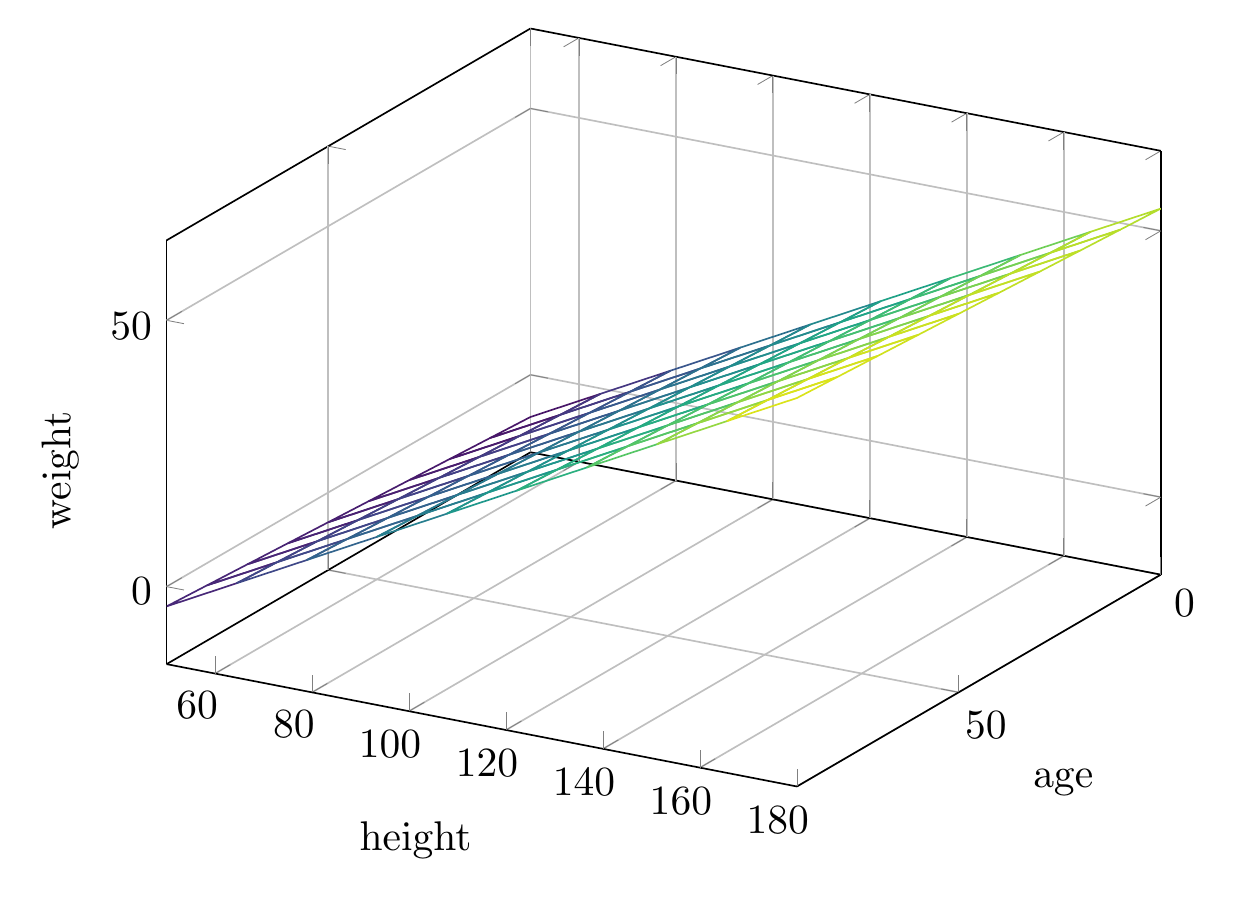
\begin{tikzpicture}[>=Stealth, scale=1.5]
        \begin{axis}[
                view={120}{30}, % 3D视角
                xlabel={age}, % x轴标签
                ylabel={height}, % y轴标签
                zlabel={weight}, % z轴标签
                grid=both, % 显示网格
                width=10cm, % 图形宽度
                height=8cm, % 图形高度
            ]


            \addplot3[
                only marks,
                scatter,
                mark=*, % 点的形状
                red
            ] coordinates \howelldata;


            \addplot3[
                mesh,
                domain=0:90,
                y domain=50:180,
                samples=10, % 控制采样的精细度
                colormap/viridis % 曲面的颜色映射
            ]
            {0.04676645038926784*x + 0.47766688346191755*y - 31.805656676953056}; % 这是回归方程 z = 2x + 3y + 1

        \end{axis}
    \end{tikzpicture}
\end{figure}

通过拟合,我们可以得到一个超平面,它大致描述了数据的分布。这个超平面的方程是 $0.04676645038926784 \cdot \text{age} + 0.47766688346191755 \cdot \text{height} - 31.805656676953056 = \hat{\text{weight}}$,它比单纯使用身高或者年龄的拟合效果都要好一些。由此还可以量化地看到,年龄与身高都会影响体重,但是年龄是弱相关,而身高是强相关,这也符合我们的日常经验。

不过正如我们之前一直在做的一样,让我们看看更为直观的几何视角。仍然用 $\bfx^0$ 表示全 $1$ 的向量,使用 $\bfx_{:1}$ 表示所有样本的第一个\textoverset{Feature}{特征}(分量),$\bfx_{:2}$ 表示所有样本的第二个特征,以此类推\footnote{记号说明:冒号表示取所有行,这是为了与 Python 中 Numpy, Torch 等库的列切片语法 $a[:, j]$ 对齐。}。那么多元线性拟合时的残差向量变为了\footnote{记号说明:在公式中我特意将常数项放到了最前面,这是为了让它和多项式拟合的形式保持一致。}
\[
    \begin{aligned}
        \bfr = \bfy - \hat \bfy = \bfy - (b \bfx^0 + w_1 \bfx_{:1} + w_2 \bfx_{:2} + \cdots + w_d \bfx_{:d})
    \end{aligned}
\]

如果回顾一下我们在多项式拟合一节的内容,就会发现这和多项式时的残差向量
\[
    \bfr = \bfy - (a_0 \bfx^0 + a_1 \bfx^1 + a_2 \bfx^2 + \cdots + a_{m} \bfx^{m})
\]

有着惊人的相似之处。细心的读者可能已经发现,如果令这些分量 $\bfx_{:1}, \bfx_{:2}, \ldots, \bfx_{:n}$ 分别为 $\bfx$ 的幂次组成的向量 $\bfx^1, \bfx^2, \ldots, \bfx^d$,那么我们得到的完完全全就是多项式拟合。这也就意味着,多项式拟合实际上可以视为多元线性拟合的一种特殊情况。

事已至此,我们似乎已经许多次遇到了这样一种情况:从一面看过去,是代数上,一组样本点上的线性拟合。但是从另一面看过去,确是在几何上找到高维空间的超平面中最接近给定点的向量。这里其实有不少精妙的数学原理\footnote{写给数学基础好的读者:这本质上体现了代数与几何的\textoverset{Duality}{对偶性}。},但是考虑到这里的主题是机器学习,我将只带读者简要地复习(或者学习)一下线性代数,更为系统性地从几种略有差距的视角\footnote{
    几种视角:
    \textoverset{Overall}{整体}解读、
    \textoverset{Row-wise}{按行}解读、
    \textoverset{Column-wise}{按列}解读、
    \textoverset{Element-wise}{按元素}解读。
}体会矩阵的本质。

在绘图讲解前,我首先要感谢\uhref{https://github.com/kenjihiranabe/The-Art-of-Linear-Algebra}{《线性代数的艺术》}{(\emph{The Art of Linear Algebra})} 这篇笔记,我第一次读到便感到文中的插图绘制非常精妙。它的思路是顺着吉尔伯特-斯特朗(Gilbert Strang)教授书籍\uhref{https://math.mit.edu/~gs/everyone/}{《写给所有人的线性代数》}{(\emph{Linear Algebra for Everyone})} 来的,我认为可以看成是一本矩阵图鉴,对理解矩阵运算有着极大的帮助。

\uhref{https://www.bilibili.com/video/BV1ys411472E}{3Blue1Brown 的线性代数系列}也是优质线性代数学习资源。这个制作精良的合集仅用不到两个小时的视频就清晰地从几何的角度讲明白了线性代数的基础知识,也是我入门线性代数的第一课。

矩阵有很多种\textoverset{Interpretation}{解读},不过我觉得大致可以按照是否把行看作一个整体以及是否把列看作一个整体来分为四类。
\begin{figure}[H]
    \centering
    \begin{tikzpicture}[>=Stealth]
        \pgfmathsetmacro{\elementsize}{0.7}
        \draw[<->] (-5, 0) node[above] {纵向切开}
        -- (5, 0) node[above] {把行视作整体};
        \draw[<->] (0, -5) node[below] {横向切开}
        -- (0, 5) node[above] {把列视作整体};
        \foreach \x in {-4, -3, -2, -1}{
                \foreach \y in {-4, -3, -2, -1}{
                        \fill [yellow] ({\x-\elementsize/2}, {\y-\elementsize/2}) rectangle ({\x+\elementsize/2}, {\y+\elementsize/2});
                    }
            }
        \foreach \x in {-4, -3, -2, -1}{
                \fill [green, opacity=0.5] ({\x-\elementsize/2}, {1-\elementsize/2}) rectangle ({\x+\elementsize/2}, {4+\elementsize/2});
            }
        \foreach \y in {-4, -3, -2, -1}{
                \fill [red, opacity=0.4] ({1-\elementsize/2}, {\y-\elementsize/2}) rectangle ({4+\elementsize/2}, {\y+\elementsize/2});
            }
        \fill [gray, opacity=0.5] ({1-\elementsize/2}, {1-\elementsize/2}) rectangle ({4+\elementsize/2}, {4+\elementsize/2});
        \node at (2.5, 2.5) {$f: \mathbb{R}^n \to \mathbb{R}^m$};
        \node at (2.5, -2.5) {$\begin{array}{c}\text{用点积探测}\\\text{输入的特征}\end{array}$};
        \node at (-2.5, 2.5) {$\begin{array}{c}\text{线性组合}\\\text{得到输出}\end{array}$};
        \node at (-2.5, -2.5) {$\begin{array}{c}\text{输入每一项对}\\\text{输出每一项的权重}\end{array}$};
    \end{tikzpicture}
\end{figure}

矩阵究竟是什么,我们的大学教了很多年,也没有完全搞清楚。从数学的角度看,可能\uhref{https://linear.axler.net/LADR4e.pdf}{Linear Algebra Done Right}的思路比较好,搞了个向量空间起手,全程以\textoverset{Map}{映射}的逻辑贯穿。但是在国内,大部分教材一上来前两章就是讲行列式的计算,教学内容逐渐搞僵化了。

既然是服务于机器学习,许多内容\footnote{许多内容:线性方程组的求解、行列式、\textoverset{Change of Basis}{基变换}、\textoverset{Eigen Decomposition}{特征分解}、\textoverset{Quadratic Form}{二次型}。}我们一概砍掉,只留下最为基础的内容。第一种视角就是作为 $\mathbb{R}^n \to \mathbb{R}^m$ 的线性映射。使用矩阵的第一个重要目的就是把一个线性映射“打包”成一个符号,毕竟只有这样才能方便地书写、推导和计算。从工科的视角看来,一个“向量”无非是一个数组,而一个“线性映射”实际上就是吃进去一个数组,吐出来另一个数组的机器\footnote{此注释写给编程基础较好的同学:这里的机器指的就是编程中的\textoverset{Function}{函数}。}。矩阵作为一个二维数组,忠实地记录了这个机器的所有参数。它的运算规则是这样的:
\[
    \begin{bmatrix}
        a_{11} & a_{12} & \cdots & a_{1n} \\
        a_{21} & a_{22} & \cdots & a_{2n} \\
        \vdots & \vdots & \ddots & \vdots \\
        a_{m1} & a_{m2} & \cdots & a_{mn}
    \end{bmatrix}
    \begin{bmatrix}
        x_1    \\
        x_2    \\
        \vdots \\
        x_n
    \end{bmatrix}
    =
    \begin{bmatrix}
        a_{11}x_1 + a_{12}x_2 + \cdots + a_{1n}x_n \\
        a_{21}x_1 + a_{22}x_2 + \cdots + a_{2n}x_n \\
        \vdots                                     \\
        a_{m1}x_1 + a_{m2}x_2 + \cdots + a_{mn}x_n
    \end{bmatrix}
\]

从输出的表达式中,我们自然引出了行的视角。如果把矩阵看作若干行:
\begin{figure}[H]
    \centering
    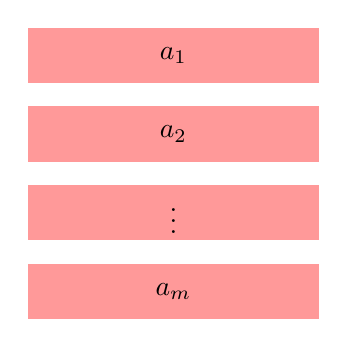
\begin{tikzpicture}
        \pgfmathsetmacro{\elementsize}{0.7}
        \foreach \y in {0, 1, 2, 3}{
                \fill [red, opacity=0.4] ({-1.5-\elementsize/2}, {\y-\elementsize/2}) rectangle ({1.5+\elementsize/2}, {\y+\elementsize/2});
            }
            \node at (0, 3) {$a_1$};
            \node at (0, 2) {$a_2$};
            \node at (0, 1) {$\vdots$};
            \node at (0, 0) {$a_m$};
    \end{tikzpicture}
\end{figure}

我们会发现输出 $y$ 的每一个分量 $y_i$ 都是输入 $x$ 与行 $a_i$ 的点积\footnote{严格地说 $a$ 是行向量,$x$ 是列向量,这中间在数学上有一些差别,是矩阵乘法而不是点积。但是在计算机存储中,因为都是一维数组,从实用的角度并不需要纠结于此,这种\textoverset{Abuse of Notation}{记号混用}就见怪不怪了。}。例如
\[
    y_1 = a_1 \cdot x = a_{11}x_1 + a_{12}x_2 + \cdots + a_{1n}x_n
\]

诚然,每一行都是一个\textoverset{Homogeneous}{齐次的}\footnote{齐次:指不带偏置(常数)项。}线性函数,它的形式也只能是这种 $x$ 的\textoverset{Weighted Sum}{加权和},但是相信一定会有读者好奇:点积衡量了两个向量的相似程度,那么这里做点积的几何意义是什么呢?答曰:探测输入的特征。

我们可以把矩阵的每一行看作一个\textoverset{Feature Detector}{特征检测器},它的方向表明了待检测的特征方向,与 $x$ 的点积则说明了这个输入在这个特征上的响应强度(通常称为\textoverset{Feature Response}{特征响应})。当 $x$ 与特征的方向相近时响应的值为正,而当 $x$ 与特征的方向相反时响应的值会为负,当 $x$ 与特征几乎无关时响应的值会接近于零。这是点积的几何特性,至少从理论上为特征提取画出了一条路径。

这时如果考虑怎么样的输入可以获得接近预期的输出呢?根据几何解释,其实就是试图找到一个输入向量,让它尽可能通过这些特征检测器,使得每一个特征检测器的响应值与预期的响应(输出的对应分量)尽可能接近,并考虑使用均方误差来“惩罚”不接近的程度,我们一开始的代数解释便是如此。

但是如果改改输出的写法,把矩阵切成若干列,我们又有了一个不同的视角,不过这里我们用 $a_{:j}$ 表示它的列:
\begin{figure}[H]
    \centering
    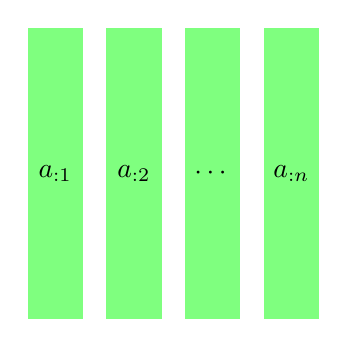
\begin{tikzpicture}
        \pgfmathsetmacro{\elementsize}{0.7}
        \foreach \x in {0, 1, 2, 3}{
                \fill [green, opacity=0.5] ({\x-\elementsize/2}, {-1.5-\elementsize/2}) rectangle ({\x+\elementsize/2}, {1.5+\elementsize/2});
            }
            \node at (0, 0) {$a_{:1}$};
            \node at (1, 0) {$a_{:2}$};
            \node at (2, 0) {$\cdots$};
            \node at (3, 0) {$a_{:n}$};
    \end{tikzpicture}
\end{figure}

这样看来,矩阵的乘法也可以写成
\[
\begin{aligned}
    Ax & = \begin{bmatrix}
        a_{:1} & a_{:2} & \cdots & a_{:n}
    \end{bmatrix}
    \begin{bmatrix}
        x_1 \\ x_2 \\ \vdots \\ x_n
    \end{bmatrix}
    \\
    &= x_1 a_{:1} + x_2 a_{:2} + \cdots + x_n a_{:n}
\end{aligned}
\]

也就是说,输出写成了输入的线性组合。这时我们在输出的空间 $\mathbb{R}^m$ 操作,而输入的空间 $\mathbb{R}^n$ 仅仅是作为权重的载体,给出了这些列向量应该以怎么样的比例组合。

这时我们要怎么考虑用输出反推合适的输入这个问题呢?随着输入的变化,输出会变为列向量的不同组合方式,正如之前所说的,我们需要在这些列向量线性组合形成的超平面上找点,让它和预期的输出尽可能接近,这就是我们在前文提到的最小二乘的几何视角。

最后一种角度则带有更为浓重的\textoverset{Distruction}{解构}\footnote{解构:哲学术语,通常指的是对一个结构或概念进行拆解、分析。}色彩:把矩阵看成一个数表,作为一个填了数字的 $m\times n$ 矩形:
\begin{figure}[H]
    \centering
    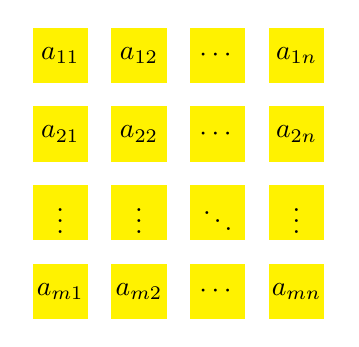
\begin{tikzpicture}
        \pgfmathsetmacro{\elementsize}{0.7}
        \foreach \x in {0, 1, 2, 3}{
                \foreach \y in {0, 1, 2, 3}{
                        \fill [yellow] ({\x-\elementsize/2}, {\y-\elementsize/2}) rectangle ({\x+\elementsize/2}, {\y+\elementsize/2});
                    }
            }
        \node at (0, 3) {$a_{11}$};
        \node at (1, 3) {$a_{12}$};
        \node at (2, 3) {$\cdots$};
        \node at (3, 3) {$a_{1n}$};
        \node at (0, 2) {$a_{21}$};
        \node at (1, 2) {$a_{22}$};
        \node at (2, 2) {$\cdots$};
        \node at (3, 2) {$a_{2n}$};
        \node at (0, 1) {$\vdots$};
        \node at (1, 1) {$\vdots$};
        \node at (2, 1) {$\ddots$};
        \node at (3, 1) {$\vdots$};
        \node at (0, 0) {$a_{m1}$};
        \node at (1, 0) {$a_{m2}$};
        \node at (2, 0) {$\cdots$};
        \node at (3, 0) {$a_{mn}$};
    \end{tikzpicture}
\end{figure}

一般来说,我们的教材都是这么引入的,但是就像我刚才提到的一样,这种理解有着一股解构的色彩。如果没有解构后重新的\textoverset{Construction}{建构}\footnote{建构:哲学术语,通常指的是对一个结构或概念进行重建、整合。},这种理解很容易让人迷失在行列式、特征值、特征向量等等复杂计算的汪洋大海中,从而忘记了矩阵的本质。那么这种解释有什么意义呢?我认为它的作用就在于 $a_{ij}$ 体现了第 $j$ 个输入对第 $i$ 个输出的权重。

让我们看看下面这个示意图:
\begin{figure}[H]
    \centering
    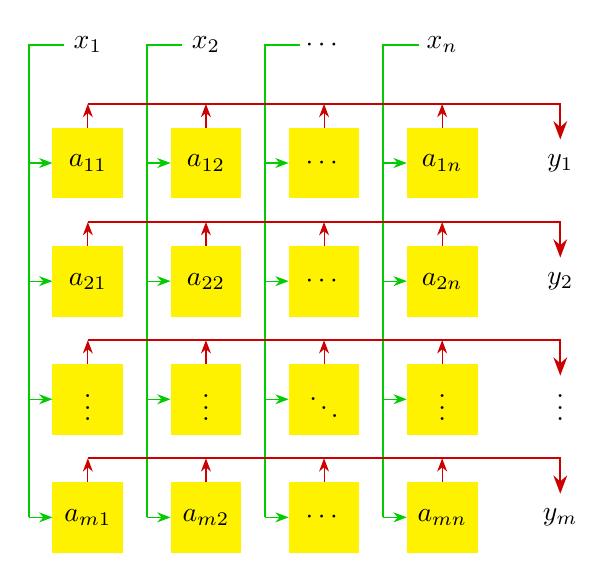
\begin{tikzpicture}[>=Stealth, scale=1.5]
        \pgfmathsetmacro{\elementsize}{0.6}
        \foreach \x in {0, 1, 2, 3}{
                \foreach \y in {0, 1, 2, 3}{
                        \fill [yellow] ({\x-\elementsize/2}, {\y-\elementsize/2}) rectangle ({\x+\elementsize/2}, {\y+\elementsize/2});
                    }
            }
        \foreach \x in {0, 1, 2, 3}{
            \draw [green!80!black, thick] ({\x - 0.2}, 4) -- ({\x - 0.5}, 4) -- ({\x - 0.5}, 0);
            \foreach \y in {0, 1, 2, 3}{
                \draw [->, green!80!black] ({\x - 0.5}, \y) -- ({\x - \elementsize/2}, \y);
            }
        }
        \foreach \y in {0, 1, 2, 3}{
            \draw [red!80!black, thick, ->] (0, {\y + 0.5}) -- (4, {\y + 0.5}) -- (4, {\y + 0.2});
            \foreach \x in {0, 1, 2, 3}{
                \draw [->, red!80!black] (\x, {\y + \elementsize/2}) -- (\x, {\y + 0.5});
            }
        }
        \node at (0, 3) {$a_{11}$};
        \node at (1, 3) {$a_{12}$};
        \node at (2, 3) {$\cdots$};
        \node at (3, 3) {$a_{1n}$};
        \node at (0, 2) {$a_{21}$};
        \node at (1, 2) {$a_{22}$};
        \node at (2, 2) {$\cdots$};
        \node at (3, 2) {$a_{2n}$};
        \node at (0, 1) {$\vdots$};
        \node at (1, 1) {$\vdots$};
        \node at (2, 1) {$\ddots$};
        \node at (3, 1) {$\vdots$};
        \node at (0, 0) {$a_{m1}$};
        \node at (1, 0) {$a_{m2}$};
        \node at (2, 0) {$\cdots$};
        \node at (3, 0) {$a_{mn}$};

        \node at (0, 4) {$x_1$};
        \node at (1, 4) {$x_2$};
        \node at (2, 4) {$\cdots$};
        \node at (3, 4) {$x_n$};

        \node at (4, 3) {$y_1$};
        \node at (4, 2) {$y_2$};
        \node at (4, 1) {$\vdots$};
        \node at (4, 0) {$y_m$};
    \end{tikzpicture}
\end{figure}

矩阵乘法可以看成这样:输入的每个分量沿着列地址线\footnote{地址线:计算机内存中的概念,虽然逻辑上内存是连续的,但是实际上内存寻址时有很多层,最底层时被选择的内存芯片是通过行和列寻址的,物理上由两条地址线输入\textoverset{Row/Column Address Strobe}{行/列地址选通信号。}}输入到每一列的所有块,由每个元素乘上对应的权重后,将结果“上传”到对应的行地址线上,最后在行地址线上的所有块累积起来得到输出的每个分量。

这个图还有另外一个很常见的呈现形式,把它看成一个无偏置的\textoverset{Linear Layer}{线性层}\footnote{线性层:在后面章节的机器学习中会成为一个基本模块,本质上就是从输入 $x$ 得到输出 $y=Ax + b$ 的过程,这里的无偏置即 $b=0$。},我们通常是这样绘制的:
\begin{figure}[H]
    \centering
    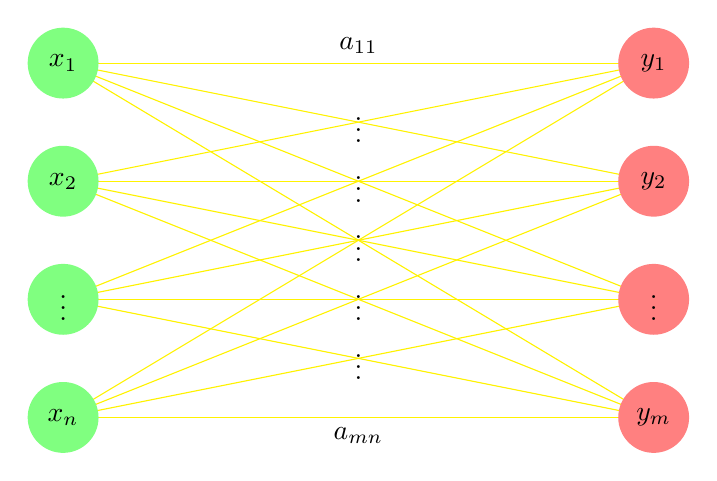
\begin{tikzpicture}[>=Stealth, scale=1.5]
        \pgfmathsetmacro{\elementradius}{0.3}
        \foreach \x in {0, 1, 2, 3} {
            \foreach \y in {0, 1, 2, 3} {
                \draw [yellow] (0, \x) -- (5, \y);
            }
        }
        \foreach \x in {0, 1, 2, 3}{
            \fill [green!50!white] (0, \x) circle (\elementradius);
        }
        \foreach \y in {0, 1, 2, 3}{
            \fill [red!50!white] (5, \y) circle (\elementradius);
        }
        \node at (0, 3) {$x_1$};
        \node at (0, 2) {$x_2$};
        \node at (0, 1) {$\vdots$};
        \node at (0, 0) {$x_n$};

        \node at (5, 3) {$y_1$};
        \node at (5, 2) {$y_2$};
        \node at (5, 1) {$\vdots$};
        \node at (5, 0) {$y_m$};

        \node[above] at (2.5, 3) {$a_{11}$};
        \foreach \y in {0.5, 1.0, ..., 2.5}{
        \node at (2.5, \y) {$\vdots$};}
        \node[below] at (2.5, 0) {$a_{mn}$};
    \end{tikzpicture}
\end{figure}

每条从 $x$ 到 $y$ 的连线都代表有一个从 $x$ 到 $y$ 的权重,我们给 $x_j$ 到 $y_i$ 的连线赋予权重 $a_{ij}$,它就表明了输入 $x_j$ 是如何影响输出 $y_i$ 的。

至此我们已经从四个有差别但是又有联系的视角理解了矩阵的行为,不过我觉得我对于不同的解释还有一点观察。当降维时,特征提取(行的视角)体现的更明显,而当升维时,特征组合(列的视角)更为重要。降维伴随着对信息的压缩和精简,通过去掉不重要的部分,更接近事物的本质。升维不仅仅是增加维度,更是通过新的空间来赋予数据提供更多的可变性。在这个过程中,每一列代表了一个基向量,整个矩阵的列向量按比例组合出高维的结果。

花了一些篇幅来复习线性代数,是时候回到多元线性拟合的问题上了。不过这次可以使用矩阵的语言来描述这个问题了。假设我们有 $n$ 组 $d$ 维的 $x$ 的取值,它们组成了一个 $n\times d$ 的矩阵 $\bfx$\,\footnote{记号说明:使用大写字母表示矩阵的比较多,但是这里为了美观和符号的一致性,我们仍然采用黑体小写字母表示所有数据点的集合。$\bfx_i$ 表示第 $i$ 个数据点,$\bfx_{:j}$ 表示所有数据点的第 $j$ 个分量,$x_{ij}$ 表示第 $i$ 个数据点的第 $j$ 个分量,因为是标量,所以采取小写。而在方程 $x\cdot w$ 中,$x,w$ 并非数据点的集合,而是变量,故虽然为向量,但是采用斜体。}。我们的目标是找到一个 $d$ 维的 $w$,使得数据集上 $x\cdot w$ 尽可能接近 $y$,现在 $\hat y$ 的表达式用点积的语言可以简洁地写为 $\hat y = x\cdot w + b$ 这种形式。

但是通过一点点技巧可以让问题更简洁,在拟合函数中,我们可以把 $b$ 合并到 $w$ 中,也就是
\[
\begin{aligned}
    \hat y &= x \cdot w + b \\
    &= x_1 w_1 + x_2 w_2 + \cdots + x_d w_d + b\\
    &= \begin{bmatrix}
        x_{1} & x_{2} & \cdots & x_{d} & 1
    \end{bmatrix}
    \begin{bmatrix}
        w_1 \\ w_2 \\ \vdots \\ w_d \\ b
    \end{bmatrix}
\end{aligned}
\]

对于样本,把所有的行并起来就变成了不需要额外添加偏置的 $\hat \bfy = \tilde \bfx \tilde w$。如果要说这个 $\tilde \bfx$ 是什么,它就是把 $\bfx$ 的每一行拼上一个 $1$:
\begin{figure}[H]
    \centering
    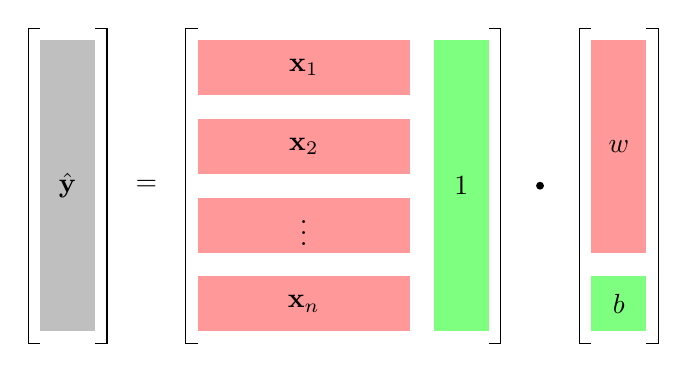
\begin{tikzpicture}
        \pgfmathsetmacro{\elementsize}{0.7}
        \fill [gray, opacity=0.5] ({-2-\elementsize/2}, {-\elementsize/2}) rectangle ({-2+\elementsize/2}, {3+\elementsize/2});
        \node at (-2, 1.5) {$\hat \bfy$};
        \draw ({-2-\elementsize/2}, -0.5) -- (-2.5, -0.5) -- (-2.5, 3.5) -- ({-2-\elementsize/2}, 3.5);
        \draw ({-2+\elementsize/2}, -0.5) -- (-1.5, -0.5) -- (-1.5, 3.5) -- ({-2+\elementsize/2}, 3.5);
        \node at (-1, 1.5) {$=$};
        \foreach \y in {0, 1, 2, 3}{
                \fill [red, opacity=0.4] ({0-\elementsize/2}, {\y-\elementsize/2}) rectangle ({2+\elementsize/2}, {\y+\elementsize/2});
            }
            \node at (1, 3) {$\bfx_1$};
            \node at (1, 2) {$\bfx_2$};
            \node at (1, 1) {$\vdots$};
            \node at (1, 0) {$\bfx_n$};
        \fill [green, opacity=0.5] ({3-\elementsize/2}, {-\elementsize/2}) rectangle ({3+\elementsize/2}, {3+\elementsize/2});
        \node at (3, 1.5) {$1$};
        \draw ({-\elementsize/2}, -0.5) -- (-0.5, -0.5) -- (-0.5, 3.5) -- ({-\elementsize/2}, 3.5);
        \draw ({3+\elementsize/2}, -0.5) -- (3.5, -0.5) -- (3.5, 3.5) -- ({3+\elementsize/2}, 3.5);
        \fill [red, opacity=0.4] ({5-\elementsize/2}, {1-\elementsize/2}) rectangle ({5+\elementsize/2}, {3+\elementsize/2});
        \fill (4, 1.5) circle (0.05);
        \node at (5, 2) {$w$};
        \fill [green, opacity=0.5] ({5-\elementsize/2}, {-\elementsize/2}) rectangle ({5+\elementsize/2}, {0+\elementsize/2});
        \node at (5, 0) {$b$};
        \draw ({5-\elementsize/2}, -0.5) -- (4.5, -0.5) -- (4.5, 3.5) -- ({5-\elementsize/2}, 3.5);
        \draw ({5+\elementsize/2}, -0.5) -- (5.5, -0.5) -- (5.5, 3.5) -- ({5+\elementsize/2}, 3.5);
    \end{tikzpicture}
\end{figure}

但是如果改成用列的视角来看待矩阵 $\tilde \bfx$,我们会发现问题变成了用 $\bfx_{:1}, \bfx_{:2}, \cdots, \bfx_{:d}$ 与 $\bfx^0$ 的线性组合来贴近 $\bfy$。
\begin{figure}[H]
    \centering
    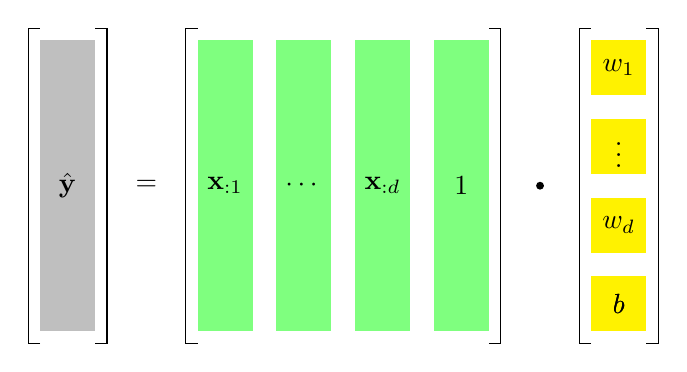
\begin{tikzpicture}
        \pgfmathsetmacro{\elementsize}{0.7}
        \fill [gray, opacity=0.5] ({-2-\elementsize/2}, {-\elementsize/2}) rectangle ({-2+\elementsize/2}, {3+\elementsize/2});
        \node at (-2, 1.5) {$\hat \bfy$};
        \draw ({-2-\elementsize/2}, -0.5) -- (-2.5, -0.5) -- (-2.5, 3.5) -- ({-2-\elementsize/2}, 3.5);
        \draw ({-2+\elementsize/2}, -0.5) -- (-1.5, -0.5) -- (-1.5, 3.5) -- ({-2+\elementsize/2}, 3.5);
        \node at (-1, 1.5) {$=$};
        \foreach \x in {0, 1, 2}{
                \fill [green, opacity=0.5] ({\x-\elementsize/2}, {0-\elementsize/2}) rectangle ({\x+\elementsize/2}, {3+\elementsize/2});
            }
            \node at (0, 1.5) {$\bfx_{:1}$};
            \node at (1, 1.5) {$\cdots$};
            \node at (2, 1.5) {$\bfx_{:d}$};
        \fill [green, opacity=0.5] ({3-\elementsize/2}, {-\elementsize/2}) rectangle ({3+\elementsize/2}, {3+\elementsize/2});
        \node at (3, 1.5) {$1$};
        \draw ({-\elementsize/2}, -0.5) -- (-0.5, -0.5) -- (-0.5, 3.5) -- ({-\elementsize/2}, 3.5);
        \draw ({3+\elementsize/2}, -0.5) -- (3.5, -0.5) -- (3.5, 3.5) -- ({3+\elementsize/2}, 3.5);
        \foreach \y in {0, 1, 2, 3}{
                \fill [yellow] ({5-\elementsize/2}, {\y-\elementsize/2}) rectangle ({5+\elementsize/2}, {\y+\elementsize/2});
            }
            \node at (5, 3) {$w_1$};
            \node at (5, 2) {$\vdots$};
            \node at (5, 1) {$w_d$};
            \node at (5, 0) {$b$};
        \fill (4, 1.5) circle (0.05);
        \node at (5, 0) {$b$};
        \draw ({5-\elementsize/2}, -0.5) -- (4.5, -0.5) -- (4.5, 3.5) -- ({5-\elementsize/2}, 3.5);
        \draw ({5+\elementsize/2}, -0.5) -- (5.5, -0.5) -- (5.5, 3.5) -- ({5+\elementsize/2}, 3.5);
    \end{tikzpicture}
\end{figure}

诶?这不是函数拟合问题吗?如果把 $\bfy$ 和 $\bfx_{:j}$ 看作是关于 $i$ 的函数(这里函数定义在 $\{1, 2, \cdots, n\}$ 上,换言之,记 $\bfy(1) = y_1, \bfy(2) = y_2, \cdots, \bfy(n) = y_n$,同理,设 $\bfx_{:j}(i) = x_{ij}$。那么我们的问题就是用 $d$ 个函数 $\bfx_{:1}(i) \sim \bfx_{:d}(i)$ 与一个常值函数 $\bfx^{0}(i) \equiv 1$ 来拟合一个给定的函数 $\bfy(i)$。

去掉常数项(或者把常数项也当成一个 $\bfx_{:d+1}$ )并把自变量 $i$ 当成一元函数拟合问题中的 $x$ 就可以发现:这与使用给定函数 $f_1(x)\sim f_d(x)$ 的线性组合,在若干数据点上拟合给定函数 $f(x)$ 这一问题没有任何差别。由此可见,用给定的函数集来拟合一个函数本质上与多元线性拟合有着完全相同的数学结构。

至此,我们至少已经初步理解了线性拟合。在这一章的最后,让我们做个总结。

\begin{itemize}
    \item 最开始我们引入了一元的线性拟合,学会了最小二乘法与最小化损失以优化参数的基本思想,也学会了如何给数据加权。
    \item 接下来来到了多项式拟合,虽然是曲线,但是如果把 $x$ 的方幂看作线性独立的分量,这仍然可以看作是一种线性拟合,在这里我们领略到了过拟合的危害,也理解了为什么要使用正则化与归一化方法。
    \item 在过拟合中,我们得到的更重要的启示是要意识到高次并不意味着万能,合适的才是最好。如果参数足以存下所有的数据,那么大概率就会过拟合。
    \item 最后我们引入了多元线性拟合,通过矩阵的不同解读,我们理解了特征提取与特征重组的逻辑。
    \item 从矩阵的行、列解读中,我们意识到多元线性拟合与函数的线性拟合本质上是一样的,这里有一种精妙的对应关系。
\end{itemize}

\begin{tcolorbox}[myrecommendbox, title=推荐阅读, breakable=false]
    \begin{itemize}
        \item The Art of Linear Algebra 这篇文章非常好,但是如果你上不去 GitHub,进这个知乎回答看也行:\\
              \textit{如何快速理解线性代数? - 丿小奇迹丨的回答 - 知乎}\\
              \url{https://www.zhihu.com/question/30726396/answer/3124578647}
            \item 这篇文章推荐给数理统计与线性代数都学的较好的读者:\\
                  \textit{回归分析|笔记整理(6)——多元线性回归(上) - 学弱猹的文章 - 知乎}\\
                  \url{https://zhuanlan.zhihu.com/p/48541799}
    \end{itemize}
\end{tcolorbox}
\newpage

\section{逻辑亦数据}
% 从程序执行的视角开始,引入数据是如何编码逻辑的
\subsection{逻辑门}

我们不妨将视角从拟合上短暂地移开,我相信理解逻辑和数据的关系多少也会帮助我们理解神经网络。读者或许好奇过,计算是如何完成的呢?在讨论这个问题之前,先来做一个约定,我们将 0 视作\textoverset{False}{假},1 视作\textoverset{True}{真}\footnote{逻辑0/1:在物理上,逻辑 0 由\textoverset{Low}{低电平}表示,逻辑 1 由\textoverset{High}{高电平}表示,TTL 和 CMOS 电路各有多种电压标准,感兴趣的读者可以自行学习电路的知识。}。先来看看几种最简单的逻辑运算。

\begin{enumerate}
    \item \textoverset{Not}{非}(数学写法:$\neg$,C 语言写法:\texttt{!},Python 写法:\texttt{not})
    
    非是一元运算符,它只有一个输入,输出与输入相反,其中
    \[
        \neg 0 = 1, \neg 1 = 0
    \]
    也就是说 $\neg x = 1 - x$,$x$ 与 $\neg x$ 是互补的。如果你看逻辑 0, 1 仍然感觉不太自然,你可以把它想成 False = not True, True = not False。

    \item \textoverset{And}{与}(数学写法:$\land$,C 语言写法:\texttt{\&\&},Python 写法:\texttt{and})
    
    与是二元运算符,它有两个输入,仅当两输入都为 1 时输出为 1,否则输出为 0,从真值表\footnote{真值表:逻辑运算的输出与输入的关系表。}就可以看出这一点:
    \[
        \begin{array}{ccc}
            \hline
            x & y & x \land y \\
            \hline
            0 & 0 & 0 \\
            0 & 1 & 0 \\
            1 & 0 & 0 \\
            1 & 1 & 1 \\
            \hline
        \end{array}
    \]
    这与乘法的结果是一样的,所以有时也会省去和的符号,使用 $xy$ 表示 $x \land y$。
    
    \item \textoverset{Or}{或}(数学写法:$\lor$,C 语言写法:\texttt{||},Python 写法:\texttt{or})
    
    或是二元运算符,它有两个输入,仅当两输入都为 0 时输出为 0,否则输出为 1,真值表如下:
    \[
        \begin{array}{ccc}
            \hline
            x & y & x \lor y \\
            \hline
            0 & 0 & 0 \\
            0 & 1 & 1 \\
            1 & 0 & 1 \\
            1 & 1 & 1 \\
            \hline
        \end{array}
    \]
\end{enumerate}

在图上这些运算一般会这样表示:
\begin{figure}[H]
    \centering
    \includegraphics[width=0.2\textwidth]{img/not_gate.png}\quad
    \includegraphics[width=0.2\textwidth]{img/and_gate.png}\quad
    \includegraphics[width=0.2\textwidth]{img/or_gate.png}
    \caption{逻辑门:从左到右分别为非门、与门、或门}
\end{figure}

看起来这只是一些非常简单的运算,但是基本上有这些就可以构建出所有的计算\footnote{所有的运算:这里指的是\textoverset{Turing Completeness}{图灵完备性},如果你想深入了解,可以在 Steam 上购买一个叫做 \uhref{https://store.steampowered.com/app/1444480/Turing_Complete/}{Turing Complete} 的硬核游戏,推荐游玩。}。例如\textoverset{Exclusive Or}{异或}运算表示两个输入中有且仅有一个为真。最粗暴简单的方法是列出它为 1 的所有情况:$(x\land \neg y) \lor (\neg x \land y)$。这样我们就可以用非、与、或门来构建出一个异或门。

虽然它可以完成“所有的运算”,但是具体来说,比如有读者可能要问,如果我想计算加法,它应该怎么办呢?既然逻辑上只有两个值,那么自然地计算机就要使用二进制来表示数字了。二进制的加法非常简单,就以 $5+3$ 为例,我们可以这样计算:
\[
    \begin{array}{rr}
        &101 \\
        + & 011 \\
        \hline
        & 1000
    \end{array}
\]

逻辑门又是如何完成这一过程的呢?我们将它拆解成一个个小问题。当加到某一位时,我们需要考虑三个数:两个加数和进位。分成 $2^3 = 8$ 种情况
\[
    \begin{array}{cccccc|cccccc}
        \hline
        \overset{\text{加数1}}{x} & \overset{\text{加数2}}{y} & \overset{\text{后方进位}}{c} & \overset{\text{二进制位}}{s} & \overset{\text{向前进位}}{c'} & \text{out} &
        \overset{\text{加数1}}{x} & \overset{\text{加数2}}{y} & \overset{\text{后方进位}}{c} & \overset{\text{二进制位}}{s} & \overset{\text{向前进位}}{c'} & \text{out}\\
        \hline
        0 & 0 & 0 & 0 & 0 & 0&
        0 & 0 & 1 & 1 & 0 & 1\\
        0 & 1 & 0 & 1 & 0 & 1&
        0 & 1 & 1 & 0 & 1 & 2\\
        1 & 0 & 0 & 1 & 0 & 1&
        1 & 0 & 1 & 0 & 1 & 2\\
        1 & 1 & 0 & 0 & 1 & 2&
        1 & 1 & 1 & 1 & 1 & 3\\
        \hline
    \end{array}
\]

每一个输出的位都可以通过输入的逻辑运算,用一定的电路连接表示,把多个电路串起来\footnote{串起来:对于加法这个例子,在网上\uhref{https://www.bing.com/search?q=\%E5\%85\%A8\%E5\%8A\%A0\%E5\%99\%A8}{搜索全加器}就可以很容易地搜到。},就可以完成加法了。本质上我们的计算机 CPU 就是由这样的门电路与接线组成的\footnote{说明:实际上制造中,与非门、或非门使用更多,因为它们有更方便制造、体积较小、功耗低等优势。}。一个 CPU 需要大量门电路组合形成,现代的 CPU 包含数十亿个门电路,而一个门又由若干个微型的晶体管构成。为了让电路精确地实现我们预期的功能,需要精准地将电路雕刻在硅片上,这就是光刻技术如此重要的原因。但是山在那,总有人会去登的。\footnote{山在那,总有人会去登:语出刘慈欣的短篇小说\uhref{https://zhiqiang.org/resource/liucixin-mountain.html}{山},写到大量的微晶体管以精妙地排布构成电路让我想起小说中的硅基生物,如果看到这里看累了不妨去看看小说放松一下吧。}

\subsection{程序是怎么执行起来的}
\subsection{位运算与bit-flag}
\newpage

\section{为什么是神经网络}
% 从函数拟合的角度引入神经网络
\subsection{神经网络:一个大的函数}

相比于\textoverset{Neural Network}{神经网络}如何实现其功能,读者或许更想问的是:为什么要用神经网络?现有的神经网络为什么用了这些方法?对于这一类问题,一个现实的回答是:机器学习是高度以实用为导向的,实验显示这样做效果更好。在现实中,我们往往要解决各种各样的问题,人类开发者以手写每一行代码创造了各种各样的程序,自动化地解决了许多问题。但很多问题难以在有限的时间内找到确定性的解决方案,例如识别图片中的物体、识别语音、自然语言处理等等。它们有一个共同点:输入的信息量巨大、关系复杂,难以用确定的规则来描述。手动规定像素范围来判断物体类型,或用固定的规则来解析自然语言显然并不现实。因此人们自然要问有没有更加自动化、灵活、智能的方法来一劳永逸地解决这些问题。人工智能的概念就此提出,人们希望让机器自己学习知识来解决问题。

虽然目前人类仍然很难说摸到了\textoverset{Artificial General Intelligence}{通用人工智能}\footnote{通用人工智能:指能像人类一样解决各种通用的问题的人工智能。}的边界,但人工智能已然在许多问题上取得了巨大成就,走出了 20 世纪末 21 世纪初被大众认为是“伪科学”的寒冬。经过\uhref{https://arxiv.org/pdf/1512.03385}{深度残差网络}在图像识别的重大突破、\uhref{https://www.davidsilver.uk/wp-content/uploads/2020/03/unformatted_final_mastering_go.pdf}{AlphaGo}学会下围棋、\uhref{https://arxiv.org/pdf/1706.03762}{Transformer}在翻译比赛取得优异成绩并引来一波生成式模型的热潮等等,人工智能就这样走向了时代的焦点。但是如果要问:为什么它这么成功?最直接的回答仍是:It works.

除了一些基础的训练方法外,其它的结构构成、参数调整等等往往都是人们有一个想法,于是就这样展开了实验。部分实验成功了,就说明这个想法是对的,从而延伸出新的调节思路。如此循环往复,形成了现在的人工智能领域。因此就模型结构而言并没有非常完备的理论,有的只能说是经验法则。

不过我想可以对解决的方法做一个简单的分类。按照参数的数量,从参数复杂到参数简单可以画出一条轴。按照模型获取经验的方式,从模型完全编码了先验经验,到通过一些例子得到经验,再到持续在与环境的互动中获取经验,可以画出另一条轴。在这里我也试图并不严谨地画出了这样一个表格。
\begin{table}[H]
\centering
\begin{tabular}{c|cccc}
\toprule
\textbf{监督方式 $\backslash$ 参数量} & \textbf{超大参数量} & \textbf{大参数量} & \textbf{小参数量} & \textbf{经典模型} \\
\midrule
\textbf{持续互动} & PPO, A3C & DQN & Q-Learning & 经典控制\\
\textbf{输入/输出对} & ResNet, Transformer & 浅层CNN & 浅层MLP & SVM \\
\textbf{无监督} & GAN, SimCLR & -------- & K-Means, KNN & PCA, t-SNE \\
\bottomrule
\end{tabular}
\end{table}
读者看到的第一反应大抵是感到看不懂。不过我也并非想让读者先学完再来看这个表格,而是希望读者看到:解决问题的方法虽然多样,但仍可根据若干指标大致分类。表中的术语有的是模型结构,有的是算法,有的是思想,而右侧的一列甚至根本就不是机器学习,对机器学习有基本了解的读者或许会认为它们可比性存疑。诚然,模型之间并没有一个实际上的绝对界限,表中划分的位置也仅是凭借我的经验评价一个模型大多数时候处于什么位置,而非绝对的准则,但我认为这样的划分是有意义的,用一种更为建设性的话来说:意义就是在混乱的世界中建构起规律,用于解决问题。

大参数量的一侧——神经网络的领域,正是本书的主题。作为神经网络的引入,有必要从更高的角度来理解以神经网络为基础的模型目标是什么。小节标题已经足以表达内容核心:先不论内部结构如何,所谓的神经网络,无非也是一个函数。所谓函数,就必然要考虑到输入和输出,或者更准确地说,我们关心的就是怎么用计算机程序对给定的输入,得到我们想要的输出。无论是连续的数据,还是按照 0 或者 1 编码为向量的标签,输入和输出都可以变为向量。因此许多问题都可以归结为一个更加狭义的、数值拟合意义上的函数拟合问题。一个\textoverset{Encoder}{编码器}将原始输入变为向量这种易于处理的形式。而对于函数的原始输出,可以通过一个\textoverset{Decoder}{解码器}将数值构成的向量变为我们想要的输出。

而再向前看,在第一章中我们已经初步了解了以线性回归为代表的一类函数拟合问题。虽然这一问题从结构上相对简单,但是从这一情境中可以抽象出函数拟合的理念:有一些输入和输出的对应关系,我们要设计一个带参数的拟合模型,调整参数,让模型的输出尽可能接近我们预期的输出,接近程度则通过一个损失函数来衡量。

因此我会把模型抽象成五个要素:\textoverset{Input}{输入}、\textoverset{Output}{输出}、\textoverset{Architecture}{模型结构}、\textoverset{Loss Function}{损失函数}和\textoverset{Optimizer}{优化算法}。输入、模型架构和具体参数决定了输出如何计算,按照损失函数计算得到的损失指导模型调整具体参数,优化算法则决定了参数如何调整。当然这样的划分只是我自己的理解,而非理解神经网络的唯一方式。这里我不打算在概念之间玩文字游戏,把机器学习中的概念倒来倒去,变成一篇又臭又长,令人看完莫名其妙、不知所云、又对实践毫无益处的文章。因此我认为画一个图串起来是最直观的方式。
\begin{figure}[H]
\centering
\begin{tikzpicture}[>=Stealth]
    \fill [cyan, opacity=0.5] (0, 0) rectangle (1, 1);
    \node at (0.5, 0.5) {$x'$};
    \node [below] at (0.5, 0) {向量输入};
    \fill [green, opacity=0.5] (4, 0) rectangle (5, 1);
    \node at (4.5, 0.5) {$y'$};
    \node [below] at (4.5, 0) {向量输出};
    \draw [->] (1.2, 0.5) -- node [above] {模型} (3.8, 0.5);
    \fill [lightgray, opacity=0.5] (8, 0) rectangle (9, 1);
    \node at (8.5, 0.5) {$l$};
    \node [below] at (8.5, 0) {损失};
    \draw [->] (5.2, 0.5) -- node [above] {损失函数} (7.8, 0.5);
    \fill [yellow, opacity=0.5] (4, 2) rectangle (5, 3);
    \node at (4.5, 2.5) {$o$};
    \node [below] at (4.5, 2) {优化器};
    \draw [->] (8.5, 1.2) -- (8.5, 2.5) -- node [above] {优化信息} (5.2, 2.5);
    \draw [->] (3.8, 2.5) -- (2.5, 2.5) -- node [left] {参数更新} (2.5, 1.2);
    \draw [dashed] (-0.6, -0.8) rectangle (9.6, 3.4);
    \fill [cyan, opacity=0.5] (-4, 0) rectangle (-3, 1);
    \node at (-3.5, 0.5) {$x$};
    \node [below] at (-3.5, 0) {输入};
    \draw [->] (-2.8, 0.5) -- node [above] {编码器} (-0.2, 0.5);
    \fill [green, opacity=0.5] (4, -3) rectangle (5, -2);
    \node at (4.5, -2.5) {$y$};
    \node [below] at (4.5, -3) {输出};
    \draw [->] (4.5, -0.6) -- node [right] {解码器} (4.5, -1.8);
\end{tikzpicture}
\end{figure}

从输入到输出再到损失的过程通常称为\textoverset{Forward Propagation}{正向传播},而从损失到参数的更新过程则称为\textoverset{Backward Propagation}{反向传播}。而这中间的模型结构常常由矩阵运算与一些\textoverset{Activation Function}{激活函数}构成的层组成。几乎可以说众多的神经网络中,只有这种传播的方式和网络的基本组成元素是相同的,如何从这些基本元素构建出好的模型则像是搭积木一样,各有各的搭法。

在这里我想简单讲讲使用矩阵运算的原因。在第一章中我们已经简单地学习了矩阵运算的基本知识,它本质上是正比例函数在向量空间中的推广,只是 $y=kx$ 中的斜率变成了一个个从输入 $x_j$ 连接到输出 $y_i$ 的权重 $w_{ij}$。从行看过去,它反映了输出的每个分量(或称为特征)是如何由输入的每个分量线性组合而成的。而从列看过去,它表明了输入的每个分量是如何影响输出的。就像一次函数有一个常数项一样,矩阵运算也有一个偏置项 $b$,运算的总体结构是 $y = wx + b$。从代数上看,它运算简单\footnote{简单:仅由简单的四则运算组成,现代 GPU 也常常提供高效的矩阵运算加速。},而从分析上看,它的输出变化光滑,容易求导\footnote{容易求导:记住这一点,这对后续反向传播等算法的实现至关重要。如果在离散的空间中操作,例如使用阶跃函数或者逻辑门,便无法借助导数来进行参数更新。}。

下一节中我们会引入激活函数,暂且不论它们的具体形式如何,它们也是一些非常简单的运算。或许读者会有疑问,这样一些简单的运算,真的有能力让神经网络胜任复杂的任务吗?\uhref{https://www.zhihu.com/question/594296903/answer/2979485641}{万能逼近定理}\footnote{万能逼近定理:指出足够大的神经网络可以以任意精度在给定范围内拟合任意的复杂函数。}虽然在理论上告诉我们它可以,却需要假定足够多的神经元,并不令人安心。所幸无数的实验表明:可以,在人类能实现的范围内,量变也可以引起质变,将一系列简单的单元堆叠起来,便可以形成复杂的行为。Philip W. Anderson\footnote{Philip W. Anderson:美国物理学家,1977 年诺贝尔物理学奖获得者。}曾说过:“More is different”,他的原意指的是物理学中,微观的规律并不能简单地推导出宏观的规律,整个系统可以表现的与单个元素完全不同,因此微观和宏观需要不同的理论来描述。但这里我们不妨借用一下,同样地认识到大量简单的数学函数也可以产生复杂的行为。在神经网络的\textoverset{Emergent}{涌现}\footnote{涌现:即增大参数量带来性能突然提升的现象。}现象中,这一事实不断地被验证。就像婴儿可以通过教育称为适应社会的成年人一样,适当的算法和足够的训练数据的确可以让神经网络学会知识。

需要说明的是,现代的机器学习库 PyTorch 与 TensorFlow 都提供了完善的参数更新机制,使得用户不必自己实现优化算法。这可以说是非常简单易用,让用户可以聚焦模型的设计。不过我仍然会解读其中的原理,并试图说明设计网络结构与优化算法的人为什么要这么做。\footnote{其中的原理:实际上人类理解的神经网络工作原理与计算机实际运行的原理或许有很大的区别,人类对现在大部分网络的理解本质上都是经过实验后进行的归纳甚至是猜测,而非从数学上严格证明。神经网络的\textoverset{Interpretability}{可解释性}仍然是很大的问题,因此很多时候人们只知道怎么样做效果好,而不“真正地”理解为什么这么做效果好,有时也被人调侃为“新时代的炼金术”。虽然有许多相关的\uhref{https://www.zhihu.com/question/320688440}{解释}来帮助人们了解神经网络中发生什么,但学界内仍然没有形成一套系统的理论。}

\newpage

\subsection{激活函数与非线性}

将 $y=wx+b$ 作为一次函数的类比应该足以说明它是很简单的一类函数。但是正如一次函数的复合 $ y = w_2(w_1x+b_1)+b_2 = w_2w_1x + (w_2b_1+b_2) $
仍然是一次函数一样,如果仅仅沉浸在矩阵运算中,我们便永远无法表达那些复杂的函数。举个最简单的例子,我们甚至无法表示输入的绝对值 $y=|x|$。因此我们需要在模型的结构中加点“非线性”,让它不仅仅局限于简单的加减乘除,专业的说法称之为\textoverset{Activation Function}{激活函数}。激活函数直接作用在每个特征上,而且函数本身通常是固定的\footnote{通常是固定的:在一些模型,例如使用可变样条函数的\uhref{https://arxiv.org/pdf/2404.19756}{KAN}中,激活函数也是可学习的,而且各个元素上的效果可能不同,但是可变的激活函数总体来说并不常见。},且总体通常呈现递增的趋势。

所谓逐元素作用,也就是说,与矩阵对特征进行组合不同,激活函数对各个分量的操作是独立的。其输入是一个向量,输出也是一个同样维数的向量。如果选定了激活函数 $f:\mathbb{R}\to\mathbb{R}$,输入为 $x = [x_1, x_2, \cdots, x_n]$,则输出为 $y = [f(x_1), f(x_2), \cdots, f(x_n)]$。

现在使用最多的激活函数是\textoverset{Rectified Linear Unit}{线性整流函数}(ReLU),虽然相对于其它激活函数,诸如 Sigmoid、tanh 等等,ReLU 其实算是晚辈,但是在关于激活函数的讨论中,\uhref{https://proceedings.mlr.press/v15/glorot1a/glorot1a.pdf}{有研究}表明它的效果更好,而后\uhref{https://proceedings.neurips.cc/paper_files/paper/2012/file/c399862d3b9d6b76c8436e924a68c45b-Paper.pdf}{AlexNet} 的成功更让它成为了主流的激活函数。虽然失去了早期其它激活函数的仿生背景,但它好用,而且非常简单。它的定义是:
\[
    \text{ReLU}(x) = \max\{0, x\} = \begin{cases}
        x, & x \geq 0 \\
        0, & x < 0 
    \end{cases}
\]

图像是这样的:
\begin{figure}[H]
\centering
\begin{tikzpicture}[>=Stealth]
    \draw [->] (-2, 0) -- (2, 0) node [below] {$x$};
    \draw [->] (0, -1) -- (0, 2) node [left] {$y$};
    \draw [domain=-2:0, smooth, variable=\x, blue, thick] plot ({\x}, 0);
    \draw [domain=0:2, smooth, variable=\x, blue, thick] plot ({\x}, {\x});
    \end{tikzpicture}
\caption{ReLU 函数图像}
\end{figure}

举一个例子就可以看出逐元素作用的含义。例如有输入向量 $x = [1, -2, 3]$,那么它经过 ReLU 激活函数的输出为 $y = [1, 0, 3]$。正的部分被保留了,而负的部分被置为 0。正如电路中的半波\textoverset{Rectifier}{整流器}一样,把负值截断了。

而它的导数也非常简单:
\[
    \frac{\mathrm{d}}{\mathrm{d} x}\text{ReLU}(x) = \begin{cases}
        1, & x > 0 \\
        0, & x < 0 
    \end{cases}
\]

读者或许会关心,那 0 这一点不可导要怎么办?其实关系不大,因为一个小数几乎不可能\footnote{几乎不可能:在最常用的 32 位浮点数中,一个数恰好取到 0 的概率大概在 $10^{-9}$ 量级。虽然在 FP8 或者 FP16 量化中恰好取到 0 的概率更大,然而实践中这单个不可导点几乎不会对训练产生影响。}在训练中恰好落在 0 上。即使有,也可以任意地选择一个值,例如 0 或者 1\footnote{0 处的导数:PyTorch 通常选择 0}。有了这样的激活函数,函数的表达能力大大就增强了。以目标 $|x|$ 为例,假设有输入 $x$,只需两个 ReLU 函数值的和就可以表示它:
\[
    |x| = \text{ReLU}(x) + \text{ReLU}(-x) = \max\{0, x\} + \max\{0, -x\}
\]

初看可能会觉得这样的表达方式有点多此一举,像是为了 $|x|$ 这盘醋专门包的饺子。但是别急,让我们把它拆解成神经网络的结构,更加结构化地看待。

最初的输入是 $x$,它先经过一个线性的函数得到 $[x, -x]$,再经过 ReLU 函数得到中间的向量 $x^{(1)} = (\max\{0, x\}, \max\{0, -x\})$,而这使用一个线性函数就可以得到 $y = |x|$。

写成矩阵的形式就有
\[
w_1 = \begin{bmatrix}
    1 \\ -1
\end{bmatrix}, b_1 = \begin{bmatrix}
    0 \\ 0
\end{bmatrix}, w_2 = \begin{bmatrix}
    1 & 1
\end{bmatrix}, b_2 = 0
\]

遂可以写成 $y = w_2 \,\text{ReLU}(w_1x + b_1) + b_2$。我认为,把这件事作为一个 toy case\footnote{toy case:玩具案例,指的是一个简单的例子,用于说明某个概念或方法。}想明白多少可以帮助理解神经网络。把矩阵的每个权重都画出来就是这样了:
\begin{figure}[H]
\centering
\begin{tikzpicture}[>=Stealth, scale=1.5]
    \node [circle, fill=white, draw, minimum size=1.2cm] (x0) at (0, 0) {$x$};
    \node [circle, fill=white, draw, minimum size=1.2cm] (x11) at (2, 1) {$x_1^{(1)}$};
    \node [circle, fill=white, draw, minimum size=1.2cm] (x12) at (2, -1) {$x_2^{(1)}$};
    \node [circle, fill=white, draw, minimum size=1.2cm] (y) at (4, 0) {$|x|$};
    \draw [->, red] (x0) -- node [above left] {$1$} (x11);
    \draw [->, blue] (x0) -- node [below left] {$-1$} (x12);
    \draw [->, red] (x11) -- node [above right] {$1$} (y);
    \draw [->, red] (x12) -- node [below right] {$1$} (y);
    \draw [dashed, thin] (1.4, -1.8) rectangle (2.6, 1.8);
    \node [above] at (2, 1.8) {中间层};
    \node at (2, 0.4) {ReLU};
    \node[lightgray] at (2, 1.6) {$+0$};
    \node[lightgray] at (2, -0.4) {$+0$};
    \node[lightgray] at (4, 0.6) {$+0$};
    \node at (2, -1.6) {ReLU};
    \end{tikzpicture}
\caption{神经网络表示 $|x|$}
\end{figure}

这看起来很简单,读者可能想问:还能不能再给力一点,看看更复杂的情况呢?当然可以。不过在看之前先抛出两个思考题:
\begin{enumerate}
    \item 试着用线性函数和 ReLU 函数表示 $y = \max\{x_1, x_2\}$,并画出它的神经网络结构图。
    \item 线性函数和 ReLU 的组合\textbf{不能}表示什么函数呢?
\end{enumerate}

在思考这个问题时,读者可以先回顾 ReLU 的性质:它的作用是将负数截断为 0,而正数保持不变。那么,能否通过适当的线性变换和 ReLU 来分辨两个数的大小呢?实际上我们可以很容易地发现
\[
    \max\{x_1, x_2\} = x_1 + \text{ReLU}(x_2 - x_1) 
\]

但是这个答案并不够好,如果直接把它画成神经网络结构图,就会发现它的结构看起来像是这样:
\begin{figure}[H]
\centering
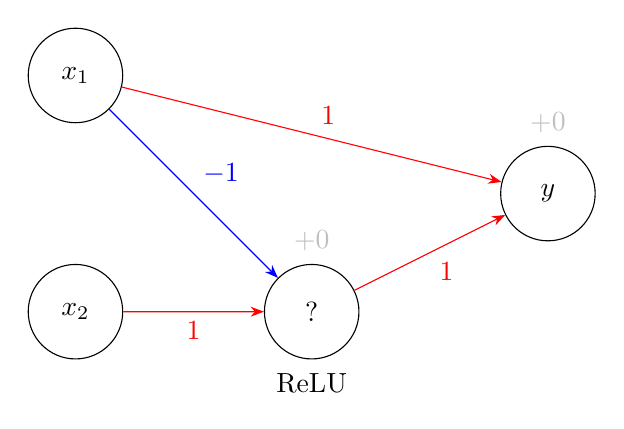
\begin{tikzpicture}[>=Stealth, scale=1.5]
    \node [circle, fill=white, draw, minimum size=1.2cm] (x01) at (0, 1) {$x_1$};
    \node [circle, fill=white, draw, minimum size=1.2cm] (x02) at (0, -1) {$x_2$};
    \node [circle, fill=white, draw, minimum size=1.2cm] (x11) at (2, -1) {$?$};
    \node [circle, fill=white, draw, minimum size=1.2cm] (y) at (4, 0) {$y$};
    \draw [->, blue] (x01) -- node [above right] {$-1$} (x11);
    \draw [->, red] (x02) -- node [below] {$1$} (x11);
    \draw [->, red] (x11) -- node [below right] {$1$} (y);
    \draw [->, red] (x01) -- node [above right] {$1$} (y);
    \node at (2, -1.6) {ReLU};
    \node[lightgray] at (2, -0.4) {$+0$};
    \node[lightgray] at (4, 0.6) {$+0$};
    \end{tikzpicture}
\caption{神经网络表示 $\max\{x_1, x_2\}$ 的一种方法}
\end{figure}

变量 $x_1$ 没有经过统一的隐藏层,而是跳过中间,直接连接到了输出层。显然就不能用一致的 $\text{ReLU}(wx+b)$ 的形式来表示了,而是要单独开一个通道来处理。而我们使用神经网络的目的本来就是用一致的方式来处理所有的输入,所以这样的表示方式并不优雅\footnote{并不优雅:与之对比,在深层神经网络网络中通常会引入看起来有些像这里的\textoverset{Shortcut Connection}{跳连接}结构,由此引出\textoverset{Residual Network}{残差网络}的概念。它看起来有些像这里的跳过中间层的结构,但那里是系统性地引入这样的连接,而不是这样对某个分量单独处理。}。

不过使用一点小小的技巧,可以把 $x_1$ 本身写成 $x_1 = \text{ReLU}(x_1) - \text{ReLU}(-x_1)$,这样一来就可以把它写成带有三个中间变量的一个网络结构了。把
\[
    \max\{x_1, x_2\} = \text{ReLU}(x_1) - \text{ReLU}(-x_1) + \text{ReLU}(x_2 - x_1)
\]

这一式子中的三个分量提出来,便可以得到
\[
\begin{aligned}
    x_1^{(1)} &= \text{ReLU}(x_1\,{\color{lightgray}+\,0x_2}) \\
    x_2^{(1)} &= \text{ReLU}(-x_1\,{\color{lightgray}+\,0x_2}) \\
    x_3^{(1)} &= \text{ReLU}(- x_1 + x_2) \\
    y &= x_1^{(1)} - x_2^{(1)} + x_3^{(1)} 
\end{aligned}
\]

偏置 $b$ 仍然为 $0$,读者可以自行试着写出对应的权重矩阵 $w$ ,按照新的写法重新绘制,这时结构图就会变成这样:
\begin{figure}[H]
\centering
\begin{tikzpicture}[>=Stealth, scale=1.5]
    \node [circle, fill=white, draw, minimum size=1.2cm] (x01) at (-1, 1.2) {$x_1$};
    \node [circle, fill=white, draw, minimum size=1.2cm] (x02) at (-1, -1.2) {$x_2$};
    \node [circle, fill=white, draw, minimum size=1.2cm] (x11) at (2, 2) {$x_1^{(1)}$};
    \node [circle, fill=white, draw, minimum size=1.2cm] (x12) at (2, 0) {$x_2^{(1)}$};
    \node [circle, fill=white, draw, minimum size=1.2cm] (x13) at (2, -2) {$x_3^{(1)}$};
    \node [circle, fill=white, draw, minimum size=1.2cm] (y) at (5, 0) {$y$};
    \draw [->, lightgray] (x02) -- node [below right] {$0$} (x11);
    \draw [->, lightgray] (x02) -- node [below right] {$0$} (x12); 
    \draw [->, red] (x01) -- node [above left] {$1$} (x11);
    \draw [->, blue] (x01) -- node [above right] {$-1$} (x12);
    \draw [->, blue] (x01) -- node [above right] {$-1$} (x13);
    \draw [->, red] (x02) -- node [below left] {$1$} (x13);
    \draw [->, red] (x11) -- node [above right] {$1$} (y);
    \draw [->, blue] (x12) -- node [above] {$-1$} (y);
    \draw [->, red] (x13) -- node [below right] {$1$} (y);
    \node [lightgray] at (2, 2.6) {$+0$};
    \node [lightgray] at (2, 0.6) {$+0$};
    \node [lightgray] at (2, -1.4) {$+0$};
    \node [below] at (2, 1.6) {ReLU};
    \node [below] at (2, -0.4) {ReLU};
    \node [below] at (2, -2.4) {ReLU};
    \draw [dashed, thin] (1.4, -2.8) rectangle (2.6, 2.8);
    \node [above] at (2, 2.8) {中间层};
    \end{tikzpicture}
\caption{神经网络表示 $\max\{x_1, x_2\}$ 的另一种方法}
\end{figure}

虽然中间的神经元多了一些,但是它的结构看起来就统一而且整齐得多了。或许有人会有疑问,这里连的线变多了,不是把事情复杂化了吗?实际上并没有,恰恰相反,把它整齐地写出来才有利于算法的数值优化。

一个有趣的事实是,如果把 True 和 False 分别视作 1 和 0,那么只需要最多这样的两层就可以表示任意的逻辑函数。例如 
\[
\begin{aligned}
    x_1 \; \text{and} \; x_2 &= \text{ReLU}(x_1 + x_2 - 1) \\
    x_1 \; \text{or} \; x_2 &= \text{ReLU}(x_1) + \text{ReLU}(x_2 - x_1) \\
    x_1 \; \text{xor} \; x_2 &= \text{ReLU}(x_1 - x_2) + \text{ReLU}(x_2 - x_1) 
\end{aligned}
\]

这至少表明逻辑可以在一定程度上编码进神经网络中,用一些可调的权重来模拟逻辑门\footnote{用权重模拟逻辑门:这里仅说明它可以,不过这么做太奢侈了,很浪费储存和计算资源。},因此从这一特例来看,求特征的交集、并集的操作确实可以自然地以权重的方式编码到网络的运算中。

推而广之,不难发现 ReLU 本质上完成的是将函数分段的操作。调整权重就可以做到在不同的区域选择不同的段,从而给出不同的表达式。虽然它在每一根区域内仍然是线性的,但却可以通过一些点上的弯折来实现非线性,表达能力比单纯的线性函数大大提高。这样的函数在数学上称为\textoverset{Piecewise Linear Function}{分段线性函数},如我们所见,ReLU 函数就提供了一种通用的方式来实现分段线性函数,从而将关于“分类”的信息编码到网络中。

那么它不能表示什么函数呢?由于其分段线性的特性,不难证明它无法完全精准地表示光滑的曲线,例如 $y = x^2$。而且可以证明,对于任何一个分段线性函数 $f(x)$,都可以找到一个常数 $c$ 使对于 $\|x\|$ 足够大的时候,$f(x) \leq c\|x\|$。从而增长速度有限,无法表示指数函数或者高次的多项式函数。

这确实体现出了它的局限性,但这必然是它的弱点吗?并不一定。一方面,虽然它本身无法\textbf{精准地表示}光滑的函数,但是只要给定一个自变量的区间,在这样的函数堆叠多层之后总是可以调整参数,做到\textbf{良好地近似}给定的函数。事实上只需要四段就可以在区间 $[-1, 1]$ 上用如下的分段线性函数来相当好地近似 $x^2$ 了,例如下面的分段线性函数 $f(x)$:
\[
    f(x) = 2\text{ReLU}(x-1) + 2\text{ReLU}(x) + 2\text{ReLU}(-x) + 2\text{ReLU}(-x-1) - 0.04 
\]

图像是这样的:
\begin{figure}[H]
\centering
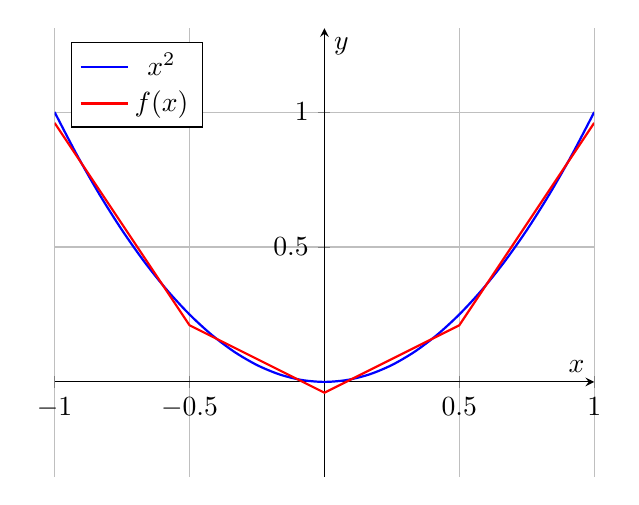
\begin{tikzpicture}[>=Stealth]
    \begin{axis}[
        axis lines=middle,
        axis equal,
        xlabel={$x$}, ylabel={$y$},
        grid=major,
        legend pos=north west
    ]
    \addplot[blue, thick, domain=-1:1, smooth] {x^2};
    \addlegendentry{$x^2$}

    \addplot[red, thick] coordinates {(-1, 0.96) (-0.5, 0.21) (0, -0.04) (0.5, 0.21) (1, 0.96)};
    \addlegendentry{$f(x)$}
    \end{axis}
\end{tikzpicture}
\caption{分段线性函数近似光滑函数}
\end{figure}

另一方面,虽然它的输出会被输入大小的一个常数倍所控制,但在很大程度上,这也避免了在第一章中多项式拟合的数值爆炸问题。此外,这提醒我们应当将模型的输入输出控制在一个范围之内。遵循这些原则,ReLU 网络的表达能力已经足够强大,能解决大多数实际问题。尽管仍有一些细节需要注意,但这并不影响我们对其整体能力的理解。

另外再提一嘴其它的激活函数。Sigmoid 函数\footnote{Sigmoid 函数:Sigmoid 来源于拉丁语,得名于其类似小写字母 sigma 变体 $\varsigma$ 的形状。}是一个 S 型函数,定义为
\[
    \text{Sigmoid}(x) = \frac{1}{1 + e^{-x}}
\]

输出随输入变化的图像是这样的,可见它把输入压缩到了 $[0, 1]$ 的范围内:
\begin{figure}[H]
\centering
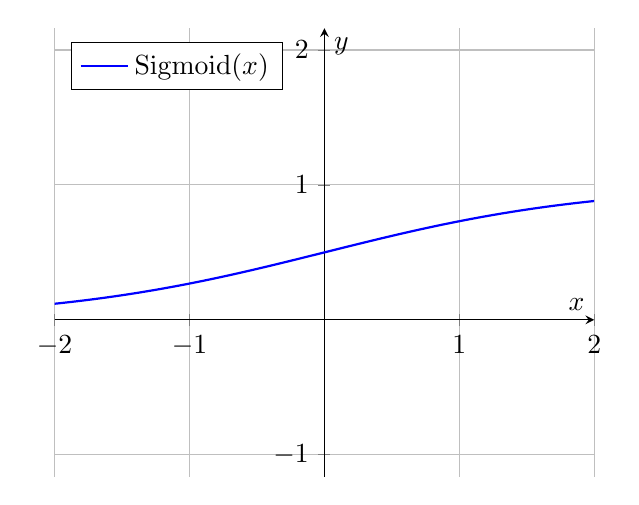
\begin{tikzpicture}[>=Stealth]
    \begin{axis}[
        axis lines=middle,
        axis equal,
        xlabel={$x$}, ylabel={$y$},
        grid=major,
        legend pos=north west
    ]
    \addplot[blue, thick, domain=-2:2, samples=100] {1/(1+exp(-x))};
    \addlegendentry{Sigmoid($x$)}
    \end{axis}
\end{tikzpicture}
\caption{Sigmoid 函数图像}
\end{figure}

tanh 函数是双曲正切函数,其定义为
\[
    \text{tanh}(x) = \frac{e^x - e^{-x}}{e^x + e^{-x}}
\]

它的图像和 Sigmoid 函数很类似,只是经过了一个伸缩和平移,输出范围是 $[-1, 1]$:
\begin{figure}[H]
\centering
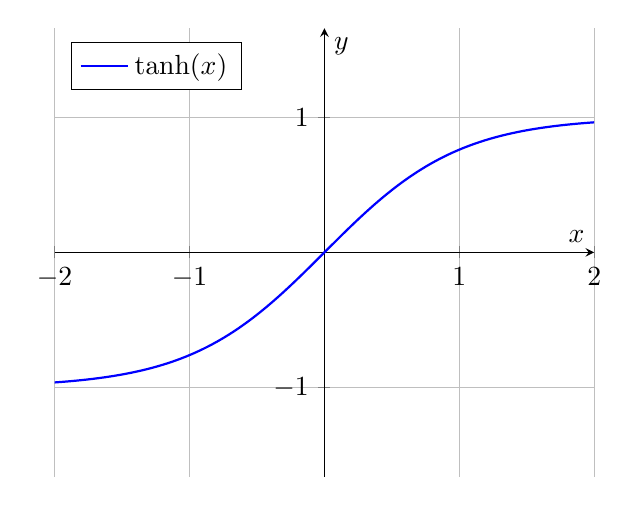
\begin{tikzpicture}[>=Stealth]
    \begin{axis}[
        axis lines=middle,
        axis equal,
        xlabel={$x$}, ylabel={$y$},
        grid=major,
        legend pos=north west
    ]
    \addplot[blue, thick, domain=-2:2, samples=100] {tanh(x)};
    \addlegendentry{tanh($x$)}
    \end{axis}
\end{tikzpicture}
\caption{tanh 函数图像}
\end{figure}

早期的研究中,它们出现在许多生物学的研究中,可以描述生物神经元的激活或者极化程度,于是人工神经网络出于仿生的考虑也使用了它们。然而它们在两端很小的导数也为优化带来了许多麻烦,导致了\textoverset{Vanishing Gradient}{梯度消失}\footnote{梯度消失:是指在深度神经网络中,由于输出随输入的变化过于小,导致信息无法有效地从输出传回输入,从而使得网络难以优化学习的现象。关于梯度的进一步介绍会在后文给出,此处可以简单理解为信息回传受阻。}的问题,后来逐渐被 ReLU 函数取代,仅在特定层要将输出限制在给定范围内时才使用。虽然近期有\uhref{https://arxiv.org/pdf/2503.10622}{研究}指出现在的优化器有能力克服这个问题,即使使用 tanh 仍然可以正常地优化,不过这也仅是一个理论上的结果,实际应用中通常认为它们仍然不如 ReLU 函数好用。从此也能看见人工智能的发展并非一帆风顺,仿生不是唯一的出路,人工的神经网络的发展和对其规律的认识必然要走过曲折的探索,才能形成一套独特而成熟的方法论。

不过 ReLU 在 $x<0$ 的区域也存在斜率为 $0$ 导致梯度消失的问题,为此人们还提出了一些变体,例如 Leaky ReLU 函数,它在 $x<0$ 的区域也有一个小的斜率,定义为
\[
    \text{Leaky ReLU}(x) = \begin{cases}
        x, & x \geq 0 \\
        \alpha x, & x < 0 
    \end{cases}
\]

上式中 $\alpha$ 是一个小的常数,通常取 $0.01$,它同样简单易于计算。还有一些较为复杂的变体,包括\textoverset{Gaussian Error Linear Unit}{高斯误差线性单元}(GELU),\textoverset{Exponential Linear Unit}{指数线性单元}(ELU) 等,都在一定程度上克服了 ReLU 导数为 $0$ 导致信息传播不畅的问题。不过这些都属于工程上的细节问题,读者可以在需要的时候再去了解。

由此我们更加具体化地认识到了神经网络的工作原理:它的基本单元由线性函数与激活函数交替组成。每一层都可以看作是对输入进行线性组合,然后通过激活函数进行非线性变换以实现更复杂的表达能力。这让网络以一种统一的方式来处理输入数据,并有能力通过调整参数拟合复杂的输出。

\newpage

\subsection{神经网络的训练}

有了前面的模块,我们已经可以搭建起简单的神经网络了,理论上通过“合适的”参数就可以拟合任意的函数了,那么“合适的”参数从何而来呢?回顾第一章中,线性拟合问题可以完全通过解析方法求解得到最优的参数,然而神经网络网络却是一个复杂的非线性函数,根本不可能对各种情况分段讨论给出解析解。那么我们是否就无能为力了呢?当然不是。通过一些手段可以让信息从数据定向地“流向”模型的参数,通过一套优化算法来调整参数,使得模型的输出尽可能地接近目标,这一过程就叫做\textoverset{Training}{训练},这一调整的过程使用的各种优化方法大多是基于\textoverset{Gradient Descent}{梯度下降法}\footnote{Gradient 词源说明:gradi 是一个拉丁语词根,意为行走,与 “步行”相关。与 progress, regress 等词中的 “gress” 是同一词根。因此从词根来看其实可以理解为在步行中下降。}的。

正如第一章中所见,拟合的好不好需要量化为损失的数值,来定量分析大小如何。而在机器学习上,我们就是借助这一可量化的评判标准——利用梯度下降算法给出了往更好的方向前进的一步。以\uhref{https://www.bilibili.com/video/BV1Ux411j7ri}{3Blue1Brown的视频}为代表的一系列科普教程中都有对这一算法的良好讲解。不过此处我仍然通过下山这个最经典的比喻来试图说明这一算法的原理。

前面我提到过,每层函数的函数需要可导,可导性就在此处显得尤为重要。即使不知道函数的总体行为,但是我们仍然可以通过导数对当前位置附近的情况形成大致的感知。就像在山上行走时,想快速下山的人并不需要知道整座山的形状,只要知道当前的坡度,就可以沿着向下的方向走。不过这一步不能走太大,在机器学习中,走太大了可能会走到山的另一边去,导数仅为优化提供了局部的信息。

在一元函数中,导数的正负可以直接指出当前的坡度是向上还是向下,局部的近似意味着对于很小的 $\Delta x$ 可以写出
\[
    \Delta y \approx f'(x_0)\Delta x
\]

看起来像是这样:
\begin{figure}[H]
\centering
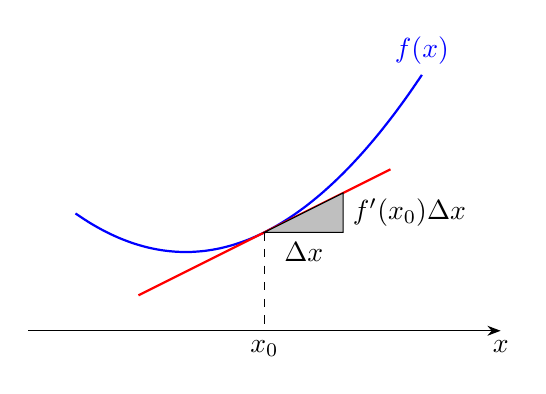
\begin{tikzpicture}[>=Stealth, xscale=2]
    \draw [thin, ->] (-1, 0) -- (2, 0) node [below] {$x$};
    % \draw [thin, ->] (0, -0.5) -- (0, 3.5) node [left] {$f(x)$};
    \draw [domain=-0.7:1.5, smooth, variable=\x, blue, thick] plot ({\x}, {\x*\x+1}) node [above] {$f(x)$};
    \draw [domain=-0.3:1.3, smooth, variable=\x, red, thick] plot ({\x}, {\x-0.25+1});
    \draw [fill=lightgray] (0.5, 1.25) -- node [below] {$\Delta x$} (1.0, 1.25) -- node [right] {$f'(x_0) \Delta x$} (1.0, 1.75) -- cycle;
    \draw [dashed, thin] (0.5, 1.25) -- (0.5, 0) node [below] {$x_0$};
    \end{tikzpicture}
\caption{一元函数的导数近似}
\end{figure}

导数反映的是切线的斜率,也就是函数在局部的变化率信息。为了让 $f(x)$ 变小,我们只需要让 $\Delta x$ 的方向与 $f'(x)$ 相反就可以了。也就是说,可以令
\[
    \Delta x = -\eta f'(x)
\]

这里的 $\eta$ 决定了一步要走多大,称为\textoverset{Learning Rate}{学习率}。如果 $\eta$ 太小,可能会走得很慢;如果 $\eta$ 太大,可能会走过头。一步步地往下走,我们的位置就像是一个小球,从斜坡上滚下去,最终停留在一个极小值\footnote{极小值:不过这个极小值可能只是山谷中的一个盆地,而非全局的最低点。}。

不过我们的神经网络毕竟有很多的参数要在同时调整,你或许想问,我们能不能固定其它的参数,只调整一个参数,把它变成一元函数来处理呢?可以是确实可以,这可以把它变为了一元函数的情况,只是这种方法太低效了,更高效且优雅的做法是联合优化它们,同时调整所有的参数。听起来很合理,但是这初听起来似乎有点玄学,毕竟我们并不知道所有的参数之间如何作用的,庞大的网络让它们之间的关系变得复杂而难以捉摸。因此我认为需要在此处引入一些多元微积分的知识,来把求导操作推广到多维,得到所谓的梯度与\textoverset{Backpropagation}{反向传播}算法。

在一元情况下,导数是这样定义的
\[
    f'(x_0) = \lim_{\Delta x\to 0} \frac{f(x_0 + \Delta x) - f(x_0)}{\Delta x}
\]

但是在输入 $x$ 是向量的情况下,数学运算并不允许除以一个向量,那么应该如何求导呢?应回看一下最初的动机:求出导数的目的是为了让它在局部能用简单的线性函数来近似。如果使用 $\mathrm{d}x$ 表示一个输入的变化量,用 $\mathrm{d}y$ 表示我们对输出结果变化量的估计,那么在一元的情况下这个式子可以简单地写成
\[
    \mathrm{d}y = f'(x_0) \mathrm{d}x
\]

而在多元情况下,应当估计每个分量的变化量如何影响输出,再把这些线性的分量叠起来,从而有线性近似
\[
    \mathrm{d}y = a_1 \mathrm{d}x_1 + a_2 \mathrm{d}x_2 + \cdots + a_n \mathrm{d}x_n
\]

而线性近似意味着在 $\mathrm{d}x$ 足够小的情况下,这一近似给出的估计 $\mathrm{d}y$ 与真实的变化量 $\Delta y$ 之间的差距是可以忽略的,也就是说
\[
    \lim_{\mathrm{d}x\to 0} \frac{\Delta y - \mathrm{d}y}{\|\mathrm{d}x\|} = 0
\]

不过上面的极限在实际应用中可以假设成立,在足够好的可导的假设下,需要关心的只是如何算出这些系数 $a_i$。对于标量函数 $f$ 和向量输入 $x$,这样的一些系数所构成的向量就叫做\textoverset{Gradient}{梯度},$f$ 对 $x$ 的梯度在 $x_0$ 处的值常记作 $\nabla_x f(x_0)$,而从根本上,它最主要的作用就是提供了线性近似 $\mathrm{d}y = \nabla_x f(x_0) \cdot \mathrm{d}x$ 的系数\footnote{说明:这里的 $\cdot$ 是向量点积,表明逐分量相乘并求和}。为了沿着网络层层回溯求出梯度,需要再引入链式法则。

设想如果 $y$ 本身并不是 $x$ 的函数,而是经过两步得到的 $x^{(1)} = f_1(x)$ 和 $y = f_2(x^{(1)})$,那么应该怎么求导呢?这一过程需要分步进行。如果从一个逐元素的视角看来,实际上是先使用 $\mathrm{d}x^{(1)}$ 来估计 $y$ 的变化量,然后再借助 $\mathrm{d}y$ 与 $\mathrm{d}x^{(1)}$ 之间的关系来估计 $\mathrm{d}x$ 对 $y$ 的影响。更为具体地说:如果能写出
\[
    \mathrm{d}y = a_1 \mathrm{d}x^{(1)}_1 + a_2 \mathrm{d}x^{(1)}_2 + \cdots + a_m \mathrm{d}x^{(1)}_m
\]

而 $\mathrm{d}x$ 对 $\mathrm{d}x^{(1)}$ 各项的影响分别是
\[
\begin{aligned}
    \mathrm{d}x^{(1)}_1 &= b_{11} \mathrm{d}x_1 + b_{12} \mathrm{d}x_2 + \cdots + b_{1n} \mathrm{d}x_n \\
    \mathrm{d}x^{(1)}_2 &= b_{21} \mathrm{d}x_1 + b_{22} \mathrm{d}x_2 + \cdots + b_{2n} \mathrm{d}x_n \\
    &\vdots \\
    \mathrm{d}x^{(1)}_m &= b_{m1} \mathrm{d}x_1 + b_{m2} \mathrm{d}x_2 + \cdots + b_{mn} \mathrm{d}x_n
\end{aligned}
\]

那么怎么把 $\mathrm{d}y$ 写成 $c_1 \mathrm{d}x_1 + c_2 \mathrm{d}x_2 + \cdots + c_n \mathrm{d}x_n$ 的形式呢?答案非常简单粗暴:把每个 $\mathrm{d}x^{(1)}_i$ 代入到 $\mathrm{d}y$ 的表达式中,就有了
\[
\begin{aligned}
    \mathrm{d}y =\, & a_1 (b_{11} \mathrm{d}x_1 + b_{12} \mathrm{d}x_2 + \cdots + b_{1n} \mathrm{d}x_n) \, + \\
    & a_2 (b_{21} \mathrm{d}x_1 + b_{22} \mathrm{d}x_2 + \cdots + b_{2n} \mathrm{d}x_n) \, + \\
    & \cdots \, +\\
    & a_n (b_{m1} \mathrm{d}x_1 + b_{m2} \mathrm{d}x_2 + \cdots + b_{mn} \mathrm{d}x_n)\\
    =\, & (a_1 b_{11} + a_2 b_{21} + \cdots + a_n b_{m1}) \mathrm{d}x_1 \,+ \\
    & (a_1 b_{12} + a_2 b_{22} + \cdots + a_n b_{m2}) \mathrm{d}x_2 \,+ \\
    & \cdots \, \,+\\
    & (a_1 b_{1n} + a_2 b_{2n} + \cdots + a_m b_{mn}) \mathrm{d}x_n
\end{aligned}
\]

由此可见,可以写出表达式
\[
\begin{aligned}
    c_j &= a_1 b_{1j} + a_2 b_{2j} + \cdots, a_m b_{mj}\\
    \mathrm{d}y &= c_1 \mathrm{d}x_1 + c_2 \mathrm{d}x_2 + \cdots + c_n \mathrm{d}x_n
\end{aligned}
\]

这表明,只要我们知道下一层计算出来的梯度 $a_i$ 和联系起两层的 $b_{ij}$,就可以将下一层的梯度“回溯”到上一层,计算出上一层的梯度 $c_j$,这种方法被称作反向传播。于是问题被进一步拆解,变成了更为细化的小问题:如何求出这里每层之间梯度传播的关系?

这里选取最简单的一层 $x^{(k)} = \text{ReLU}(w x^{(k-1)} + b)$ 来说明,其中 $w$ 是权重矩阵,$b$ 是偏置。我们需要理解 $\mathrm{d}x^{(k)}_i$ 应当如何表示。不过这里需要注意一点,在求导时不但要考虑 $x^{(k)}$ 的变化量,还要考虑 $w$ 和 $b$ 的变化量,因为 $w$ 和 $b$ 作为参数也会影响到 $x^{(k)}$ 的值,更是我们希望调整的对象。

首先写出 $x^{(k)}_i$ 的表达式
\[
    x^{(k)}_i = \text{ReLU}(w_{i1} x^{(k-1)}_1 + w_{i2} x^{(k-1)}_2 + \cdots + w_{in} x^{(k-1)}_n + b_i)
\]

接下来分类讨论,在 $\text{ReLU}$ 内部小于等于 0 的情况下,因为输入有微小变化时输出仍然为 0,所以
\[
    \mathrm{d}x^{(k)}_i = 0
\]

而当其输入大于 0 时,ReLU 可以去除掉,即变为
\[
\begin{aligned}
    \mathrm{d}x^{(k)}_i &= \mathrm{d}(w_{i1} x^{(k-1)}_1 + w_{i2} x^{(k-1)}_2 + \cdots + w_{in} x^{(k-1)}_n + b_i) \\
    &= w_{i1} \mathrm{d}x^{(k-1)}_1 + w_{i2} \mathrm{d}x^{(k-1)}_2 + \cdots + w_{in} \mathrm{d}x^{(k-1)}_n \\
    &\qquad +x^{(k-1)}_1 \mathrm{d}w_{i1} + x^{(k-1)}_2 \mathrm{d}w_{i2} + \cdots + x^{(k-1)}_n \mathrm{d}w_{in} + \mathrm{d}b_i \\
    &= w_{i:} \cdot \mathrm{d}x^{(k-1)} + x^{(k-1)} \cdot \mathrm{d}w_{i:} + \mathrm{d}b_i
\end{aligned}
\]

这里仍然沿用了向量的点积表示法,$w_{i:}$ 表示 $w$ 的第 $i$ 行。由此也可以看出 ReLU 的好处:使用它作为激活函数的梯度回溯非常方便。

这里我们会发现梯度信息发生了一个“分岔”,一部分信息传递给了 $x^{(k-1)}$,另一部分则传递给了 $w$ 和 $b$。传递给 $w$ 和 $b$ 的信息将在后续用于更新参数,而传递给 $x^{(k-1)}$ 的信息则会继续向后传递求出离结果更远、离输入更近的层的参数梯度。直到传递到输入层,最终得到所有参数的梯度,关于原始输入 $x$ 的输入则会被丢弃\footnote{丢弃:因为我们并不需要对输入进行调整,只需要对参数进行调整。不过一些研究表明,观察输入的梯度信息可以帮助我们理解模型认为哪些特征更加重要。}。这个过程看起来像是这样,如果说正向计算是把参数信息参与到计算中,一步步计算得到最终的结果(由于我们希望最小化损失,所以在模型的最终输出之后还有一个箭头表示损失函数):
\begin{figure}[H]
\centering
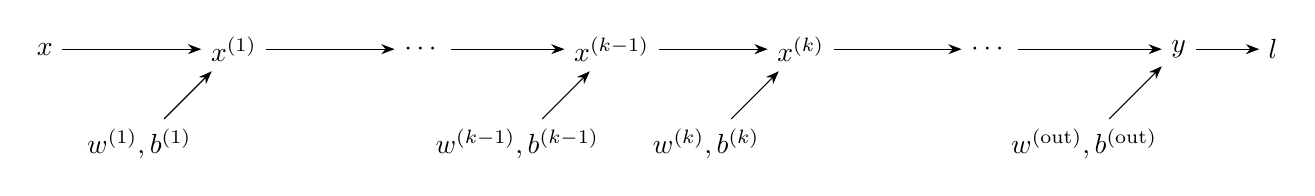
\begin{tikzpicture}[>=Stealth, scale=1.2]
    \node (x) at (0, 0) {$x$};
    \node (x1) at (2, 0) {$x^{(1)}$};
    \node (x2) at (4, 0) {$\cdots$};
    \node (x3) at (6, 0) {$x^{(k-1)}$};
    \node (x4) at (8, 0) {$x^{(k)}$};
    \node (x5) at (10, 0) {$\cdots$};
    \node (y) at (12, 0) {$y$};
    \node (w1) at (1, -1) {$w^{(1)},b^{(1)}$};
    \node (w3) at (5, -1) {$w^{(k-1)},b^{(k-1)}$};
    \node (w4) at (7, -1) {$w^{(k)},b^{(k)}$};
    \node (w5) at (11, -1) {$w^{(\text{out})}, b^{(\text{out})}$};
    \node (loss) at (13, 0) {$l$};
    \draw [->] (x) -- (x1);
    \draw [->] (x1) -- (x2);
    \draw [->] (x2) -- (x3);
    \draw [->] (x3) -- (x4);
    \draw [->] (x4) -- (x5);
    \draw [->] (x5) -- (y);
    \draw [->] (w1) -- (x1);
    \draw [->] (w3) -- (x3);
    \draw [->] (w4) -- (x4);
    \draw [->] (w5) -- (y);
    \draw [->] (y) -- (loss);
\end{tikzpicture}
\caption{正向计算}
\end{figure}

那么反向传播就是考虑损失变化的估计量 $\mathrm{d}l$,并将它的梯度信息经由 $\mathrm{d}y$ 和各个中间计算结果 $\mathrm{d}x^{(k)}$ 逐层传递回去,直到输入层。
\begin{figure}[H]
\centering
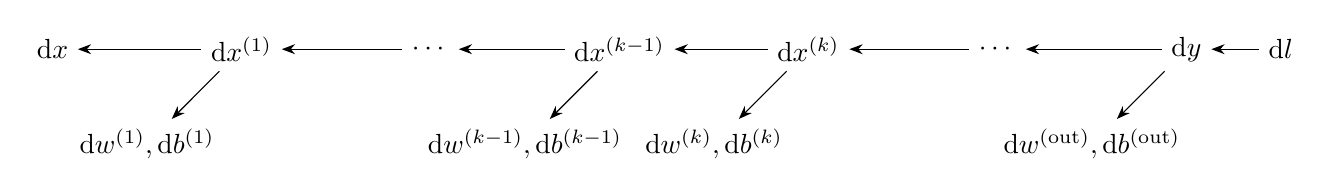
\begin{tikzpicture}[>=Stealth, scale=1.2]
    \node (x) at (0, 0) {$\mathrm{d}x$};
    \node (x1) at (2, 0) {$\mathrm{d}x^{(1)}$};
    \node (x2) at (4, 0) {$\cdots$};
    \node (x3) at (6, 0) {$\mathrm{d}x^{(k-1)}$};
    \node (x4) at (8, 0) {$\mathrm{d}x^{(k)}$};
    \node (x5) at (10, 0) {$\cdots$};
    \node (y) at (12, 0) {$\mathrm{d}y$};
    \node (w1) at (1, -1) {$\mathrm{d}w^{(1)},\mathrm{d}b^{(1)}$};
    \node (w3) at (5, -1) {$\mathrm{d}w^{(k-1)},\mathrm{d}b^{(k-1)}$};
    \node (w4) at (7, -1) {$\mathrm{d}w^{(k)},\mathrm{d}b^{(k)}$};
    \node (w5) at (11, -1) {$\mathrm{d}w^{(\text{out})}, \mathrm{d}b^{(\text{out})}$};
    \node (loss) at (13, 0) {$\mathrm{d}l$};
    \draw [<-] (x) -- (x1);
    \draw [<-] (x1) -- (x2);
    \draw [<-] (x2) -- (x3);
    \draw [<-] (x3) -- (x4);
    \draw [<-] (x4) -- (x5);
    \draw [<-] (x5) -- (y);
    \draw [<-] (w1) -- (x1);
    \draw [<-] (w3) -- (x3);
    \draw [<-] (w4) -- (x4);
    \draw [<-] (w5) -- (y);
    \draw [<-] (y) -- (loss);
\end{tikzpicture}
\caption{反向传播}
\end{figure}

在图中看到从 $\mathrm{d}x^{(k)}$ 指向 $\mathrm{d}x^{(k-1)}$ 或者 $\mathrm{d}w^{(k)}, \mathrm{d}b^{(k)}$ 的箭头时,它指的是关于 $x^{(k)}$ 的梯度信息被传递到了 $x^{(k-1)}$ 和 $w^{(k)}, b^{(k)}$ 上。上面的图只是下面表达式的一个形象说明(这里用 $g_x^{(k)}$ 表示对 $x^{(k)}$ 的梯度,同理定义对 $w$ 和 $b$ 的梯度符号)
\[
\begin{aligned}
    \mathrm{d}l &= g_y \cdot \mathrm{d}y \\
    &= g_x^{(\text{out})} \cdot \mathrm{d}x^{(\text{out})} + g_w^{(\text{out})} \cdot \mathrm{d}w^{(\text{out})} + g_b^{(\text{out})} \cdot \mathrm{d}b^{(\text{out})} \\
    &= (\text{向前展开这一部分}) + g_w^{(\text{out})} \cdot \mathrm{d}w^{(\text{out})} + g_b^{(\text{out})} \cdot \mathrm{d}b^{(\text{out})} \\
    &= g_x^{(k)} \cdot \mathrm{d}x^{(k)} + g_w^{(k)} \cdot \mathrm{d}w^{(k)} + g_b^{(k)} \cdot \mathrm{d}b^{(k)} \\
    & \qquad+ \cdots + g_w^{(\text{out})} \cdot \mathrm{d}w^{(\text{out})} + g_b^{(\text{out})} \cdot \mathrm{d}b^{(\text{out})}\\
    &= g_x^{(k-1)} \cdot \mathrm{d}x^{(k-1)} + g_w^{(k-1)} \cdot \mathrm{d}w^{(k-1)} + g_b^{(k-1)} \cdot \mathrm{d}b^{(k-1)} \\
    & \qquad+ g_w^{(k)} \cdot \mathrm{d}w^{(k)} + g_b^{(k)} \cdot \mathrm{d}b^{(k)} + \cdots \\
    &\qquad + g_w^{(\text{out})} \cdot \mathrm{d}w^{(\text{out})} + g_b^{(\text{out})} \cdot \mathrm{d}b^{(\text{out})}\\
    & = \cdots \\
    & = g_x \cdot \mathrm{d}x \\
    & \qquad + g_w^{(1)} \cdot \mathrm{d}w^{(1)} + g_b^{(1)} \cdot \mathrm{d}b^{(1)} \\
    & \qquad + g_w^{(2)} \cdot \mathrm{d}w^{(2)} + g_b^{(2)} \cdot \mathrm{d}b^{(2)} \\
    & \qquad + \cdots \\
    & \qquad + g_w^{(\text{out})} \cdot \mathrm{d}w^{(\text{out})} + g_b^{(\text{out})} \cdot \mathrm{d}b^{(\text{out})}\\
\end{aligned}
\]

随着式子每次将第一项不断地展开,树状的计算图也从计算结果的终点不断向前回溯,最终在每个终止节点处得到对每个分量的梯度信息。理论上只需要手动维护这个图的状态就能完成反向传播的计算,不过实际应用中已经有了非常方便的自动求导工具,现代的机器学习库 PyTorch 和 TensorFlow 都有类似的功能,它们都会在内部维护一个计算图,自动地完成反向传播的计算。以 PyTorch 为例,用户不需要关心如何维护这个图,只需要设置 \texttt{requires\_grad} 属性为 \texttt{True},在计算后对损失调用 \texttt{backward} 方法,就能自动地完成反向传播的计算。

在训练时数据点通常是固定的,所以可以直接令 $\mathrm{d}x = 0$,这样前面的梯度信息就仅留下与待优化的参数相关的部分
\[
\begin{aligned}
    \mathrm{d}l &= g_w^{(1)} \cdot \mathrm{d}w^{(1)} + g_b^{(1)} \cdot \mathrm{d}b^{(1)} \\
    &\qquad + g_w^{(2)} \cdot \mathrm{d}w^{(2)} + g_b^{(2)} \cdot \mathrm{d}b^{(2)} \\
    &\qquad + \cdots \\
    &\qquad + g_w^{(\text{out})} \cdot \mathrm{d}w^{(\text{out})} + g_b^{(\text{out})} \cdot \mathrm{d}b^{(\text{out})}\\
\end{aligned}
\]

而如果我们再做一层抽象,把这一堆参数塞到一个叫做 $\theta$ 的向量中,那么就可以把上面的式子写成
\[
    \mathrm{d}l = \nabla_\theta l \cdot \mathrm{d}\theta
\]

其中 $\nabla_\theta l$ 就是损失函数 $l$ 对参数 $\theta$ 的梯度,其各个分量表明了损失函数对每个参数的敏感程度。而仿照一元函数下山的做法,同样可以按照如下的方式沿着“下山最快的方向”来更新参数
\[
    \mathrm{d}\theta^* = -\eta \nabla_\theta l
\]

从图形上看,这个过程是垂直于等高线的方向在向下走,最终停留在一个极小值处。或许初看会觉得这一优化方法和等高线并不相关,但如果仔细想想就会发现,实际上等高线的形状就是损失函数的等值线,而沿着等值线的切线方向意味着
\[
    \mathrm{d}l = \nabla_\theta l \cdot \mathrm{d}\theta = 0
\]

前一个部分是梯度的方向,而令上式等于 $0$ 成立的方向 $\mathrm{d}\theta$ 就是等高线的切线方向。两个向量的内积为 $0$ 意味着它们是垂直的,用心观察的读者或许会发现,地图上的水系与等高线交汇之处,两条线往往是垂直的,水往低处走是一种自然的梯度下降。

在实际的神经网络中通常有数万乃至数亿个参数,在这样庞大的参数空间中梯度下降虽然有着下降最快的方向的理论支持,但想象一个高维空间已经足够困难,再去想它里面的等高线是什么样子就更是难上加难,所以为了便于理解,还是看一个低维空间中非常简单的样例来帮助理解。

以一个简单的函数 $f(\theta) = 2\theta_1^2 + \theta_2^2$ 为例,假设从 $(1, 1)$ 处开始迭代,取每次更新的 $\eta = 0.1$,因为 $\mathrm{d}f(\theta) = 4\theta_1 \mathrm{d}\theta_1 + 2\theta_2 \mathrm{d}\theta_2$,所以在第一步梯度为 $(2\theta_1, \theta_2) = (4, 2)$,取 $\mathrm{d}\theta^* = -\eta \nabla_\theta f$ 可以得到下一步的 $\theta$。进行 10 次迭代后,得到的点在等值线图上会按照如下图所示的方式移动,可以看到每次更新的 $\theta$ 都是垂直于等高线线的方向向下走的,逐渐逼近最优解 $(0, 0)$
\begin{figure}[H]
\centering
\includegraphics[width=0.7\textwidth]{img/gradient_descent.png}
\caption{梯度下降}
\end{figure}

不过同时我想也要给出一个错误样例说明学习率 $\eta$ 调太大会发生什么,假设刚才的例子中我们把 $\eta$ 调到 0.5, 就会发现它直接跳过极小值,跳到了空间中的对边,之后就在 $(-1, 0)$ 和 $(1, 0)$ 之间来回震荡了起来,无法收敛。
\begin{figure}[H]
\centering
\includegraphics[width=0.7\textwidth]{img/gradient_descent_0.5.png}
\caption{学习率设置不当的梯度下降}
\end{figure}

这个现象在高维空间中也会发生,如果学习率 $\eta$ 过大,常常会观察到 loss 在某个值附近反复震荡,无法收敛。

在实际有各种不同的梯度下降方法,最简单的是\textoverset{Stochastic Gradient Descent}{随机梯度下降法}(SGD),它的基本思想是每次只随机抽取部分数据来计算梯度,来更新参数。这样做的好处是每次只需要计算一小部分数据,速度快;坏处是每次计算的梯度并不准确,可能会导致参数在最优解附近震荡。有的为了加速收敛速度,使用\textoverset{Momentum}{动量法},将梯度信息不作为速度,而作为加速度来更新参数,让它能快速冲下坡。还有的使用\textoverset{Adaptive Momentum Method}{自适应动量法}(Adam),在每次更新时考虑了历史梯度信息的影响,来调整学习率。这些方法都以各自的方式帮我们找到了更好的参数更新方式,来加速收敛速度。不过动量也不是越大越好,正如学习率不是越大越好一样,过大的动量会导致参数在最优解附近震荡,甚至无法收敛。

\newpage

\subsection*{动手实践:简单的网络实践}

为了让读者对训练神经网络形成一个大概的感知,这里我会用一个极其简单的例子来说明如何训练一个神经网络。而我们的目标就是:拟合一个一元函数 $f(x) = \sin 2x$,其中 $x \in [-5, 5]$。不过为了实现这个目标,需要先简单讲一下 Python 中的数组操作。

Python 中内置的数组类型是列表,它是动态的,可以在运行时改变长度,这不同于 C 语言中为数组分配一块内存空间并储存指定类型元素。而 Python 列表中的“元素”也实际上是对象的引用。虽然原则上通常推荐用列表存储相同类型的元素\footnote{通常推荐:写类型标注时通常把列表的类型标记为 \texttt{list[T]},其中 \texttt{T} 是元素的类型,例如 \texttt{int}。},但在运行中,这类强制的要求并不存在。与 C 等语言不同的是,Python 为了实现重载符,其中的四则运算是通过调用某些特定的函数实现的\footnote{四则运算:例如 $a + b$ 实际上是调用了 \texttt{a.\_\_add\_\_(b)} 函数来实现的,仅加法这一个操作就要经过多层函数调用的包装,比 C 语言的加法慢了大概一到两数量级。},如果想在列表实现向量运算,在遍历列表的过程中就需要不停地检查对象的类型并调度对应的方法。打个比方,就像是一个工程师虽然知道生产的每一个环节,但拿到一个工件后也要先检查它的类型才能决定用什么工具来加工它。能处理的东西确实是灵活了,但是另一面是效率低下了。而与之对比的是流水线工人,他们面对的工件和工序是完全确定的,不需要检查工件的类型,只需要按照固定的流程来加工就可以了,省去了分析的时间,而且也方便同时上很多人来加工\footnote{多个人加工:指对于算术运算,CPU 中有指令可以并行地执行。}。

用 Python 原生的运算来做数值运算显然不够高效,但是 Python 的精髓就在于它的灵活性和可扩展性。可以说如果没有丰富的第三方库,Python 就不可能发展成今天这样一个强大的语言。在数值计算这一块的基石就是 NumPy,自其 2006 年发布 1.0 版本\footnote{1.0 版本:虽然对于 NumPy 来讲是 1.0 版本,不过它是在历史更久远的 Numeric 和 Numarray 两个已有的数值运算库基础上,为了统一数组运算,作为科学计算库 SciPy 的一个核心模块开发的。}开始,Python 社区内就开始广泛地使用,已经成为了 Python 进行数值计算的\textoverset{De Facto Standard}{事实标准}\footnote{事实标准:指虽然没有官方强制规定要用 NumPy,但 Python 社区内几乎所有教程、科研工作、乃至工业界都在使用它(或依赖它的其它模块),它成为了“数组运算”的通用接口标准。},重塑了整个生态\footnote{生态:例如 SciPy 和 matplotlib 分别作为科学运算库和绘图库开发早于 NumPy,但是后来它们的底层和接口都改为使用 NumPy。在社区对矩阵运算的庞大需求的推动下,连一向谨慎添加新语法的 Python 官方都专门引入了\uhref{https://peps.python.org/pep-0465/}{PEP 465 提案},早在 Python 3.5 就引入了额外的 \texttt{@} 运算符来表示矩阵乘法。}。不少人都\uhref{https://www.zhihu.com/question/645463253}{认为} NumPy 设计很好,在运算速度顶级的同时其语法和 Python 的语法风格保持了一致,同时还提供了清晰的接口和丰富的功能。有不少的优质教程可以帮助读者快速上手,\uhref{https://numpy.org/doc/stable/user/absolute_beginners.html}{NumPy 官方的初学者指南}已经是一份非常清晰的教程,其中引用的部分图片取自\uhref{https://jalammar.github.io/visual-numpy/}{NumPy 的图形化展示},即使单独看这一篇图形化教程也很好。只要用心搜索,中文互联网上亦不乏相关的优质资料,\uhref{https://zhuanlan.zhihu.com/p/396444973}{一些知乎上文章}的清晰度与丰富度也已经可以媲美官方教程,让没有经验的读者也可以快速理解 NumPy 的数组接口设计。

虽有珠玉在前,众多的教程已清晰教会了我们如何使用基础的数组操作,但我还是决定简单地讲一下数组化运算的逻辑。第一条原则是数组中的元素类型是相同的,通常 NumPy 会自动推导\footnote{自动推导:比如整型数组会变成 int64,浮点数组变成 float64。但也可以手动指定 dtype,以防不符合预期,例如如果数据点是整数但是希望参与 64 位浮点运算,那么也可以手动指定数据为 float64 类型。}\textoverset{Data Type}{数据类型}(即 dtype 参数)。第二条则是对于加减乘除这样的四则运算和 NumPy 中提供的所有一元函数(例如 sin, cos, exp 等),运算都是逐个进行的。例如两个 64 位浮点数类型的数组四则运算的结果如下。
\begin{minted}[bgcolor=gray!15, frame=single, framesep=10pt, baselinestretch=1.2]{python}
import numpy as np
x = np.array([1, 2, 3], dtype=np.float64)
y = np.array([4, 5, 6], dtype=np.float64)

print(x + y) # [5. 7. 9.]
print(x - y) # [-3. -3. -3.]
print(x * y) # [ 4. 10. 18.]
print(x / y) # [0.25 0.4  0.5 ]
\end{minted}

与经典的向量操作对比,加减法都完全相同。但是读者或许会感到疑惑,向量点积应该返回一个标量,而向量间并未定义除法。乘除法为什么要这么定义呢?因为数组不仅仅是高维空间中的一个向量,它同样可以用于表示一个函数在每一点上的取值\footnote{函数取值:这里的函数是广义上的,例如图像也可以看成是一个关于空间位置 $(i, j)$ 的二元函数,其中 $i,j$ 分别表示一个像素点的行号、列号。乘 mask 就是一个典型的逐像素作用的例子。}。逐点的乘除法不过是 $f(x) = g(x) h(x)$ 和 $f(x) = g(x) / h(x)$ 在有限个点上的表示。按传统的写法,需要通过一个循环遍历所有的 $x$ 并写入每个点的运算结果,逐元素运算则省去了这样手动遍历的麻烦。不过 \texttt{*} 用于逐元素乘法不代表无法进行想要的的点积运算。在上面的例子中,如果想计算两个向量的点积,只需 \texttt{x @ y} 或者更为明确的 \texttt{x.dot(y)} 就可以了。

了解了 NumPy 的基本原理后,获得 $f(x) = \sin 2x$ 在 $[-5, 5]$ 的样本就非常简单了。\texttt{np.linspace} 可以在给定的闭区间上均匀地采样指定的点,例如如果我们希望在 $[-5, 5]$ 上均匀采样 200 个点,导入 numpy 后只需要两行代码就能得到预期的样本:
\begin{minted}[bgcolor=gray!15, frame=single, framesep=10pt, baselinestretch=1.2]{python}
import numpy as np
x = np.linspace(-5, 5, num=200)
y = np.sin(2 * x)
\end{minted}

数据已经准备好,再下一步则是搭建一个用来拟合的神经网络了。NumPy 的数组操作很好、很优雅,但是要搭建神经网络还少一层包装。只需要回忆下训练的过程就会发现,参数更新时需要求出各个环节的梯度,而计算第 $k$ 层的参数梯度需要用到上一层的输出 $x^{(k - 1)}$ 和下一层传回的梯度 $g_x^{(k)}$。也就是说为了计算梯度,数据在正向传播的过程中需要留下“痕迹”。计算进入下一层并不能直接将它们丢弃,而是还要储存直到到梯度计算与权重更新之后才能删除。诚然,其中的许多步骤可以手动推导:写出解析的表达式,自己维护一个表用于暂存这些状态,然后手动计算梯度。但是手动计算\textoverset{Gradient Function}{梯度函数}的时代已经过去了,从最快上手的角度来看,PyTorch 中\textoverset{Automatic Gradient}{自动微分}系统的包装已经很完备,让我们网络结构就能通过样本自动完成梯度计算与优化了。学会钻木取火也许对荒野求生有很大作用,但我们作为学习做饭的现代人类,没有理由不直接打开家里的天然气灶。

PyTorch 有着类似 NumPy 的数组接口,但多了许多对网络的包装。常见的用法只需要在自定义模块时继承 \texttt{torch.nn.Module},并重写\textoverset{Initialization}{初始化}方法 \texttt{\_\_init\_\_} 和正向计算方法 \texttt{forward} 即可,将求导和参数更新的一切交给 PyTorch 的自动微分系统和优化器来处理。例如对于拟合 $f(x) = \sin 2x$ 的例子,只需要定义三层足矣:$1\to 10\to 10\to 1$\footnote{这样的中间层数量和规律并非是固定的,这里仅是随意的选择。},每一层都是一个带偏置的线性层,在中间两层加上 Leaky ReLU 激活函数并取 $\alpha = 0.1$\footnote{$\alpha$:含义可以回顾本章第一节激活函数。}。最后一层的输出是一个标量,表示对 $f(x)$ 的预测值。定义网络的过程如下:
\begin{minted}[bgcolor=gray!15, frame=single, framesep=10pt, baselinestretch=1.2]{python}
import torch
import torch.nn as nn

class SimpleModel(nn.Module):
    def __init__(self):
        super().__init__()  # Initialize the parent class
        self.linear1 = nn.Linear(1, 10)
        self.linear2 = nn.Linear(10, 10)
        self.linear3 = nn.Linear(10, 1)
        self.leaky_relu = nn.LeakyReLU(negative_slope=0.1)
    def forward(self, x):
        x = self.leaky_relu(self.linear1(x))
        x = self.leaky_relu(self.linear2(x))
        x = self.linear3(x)
        return x
\end{minted}

最上面的 \texttt{SimpleModel(nn.Module)} 表示我们定义的模型继承了 PyTorch 中的模块基类,\texttt{nn.Linear} 表示线性层。\texttt{forward} 作为模型调用的正向计算过程,通过 \texttt{model(x)} 调用时会自动触发 \texttt{forward} 的计算。

不过有一点重要的是调用 \texttt{model(x)} 时,因为一次训练时需要用到多个样本,所以输入的 $x$ 需要是一个二维数组,第一维表示样本数,第二维表示每个样本的特征数。对一元函数来说,特征数就是 $1$,样本数则是我们在前面准备的 $200$ 个点。为了让 PyTorch 能够正确地处理这个数据,我们需要将它转换为一个二维数组。可以使用 \texttt{x.reshape(-1, 1)} 来实现这个功能,其中 \texttt{-1} 表示自动推导这一维的大小,而 \texttt{1} 则表示第二维的大小为 $1$。

至于损失函数与优化器:使用均方误差作为损失函数,\texttt{torch.nn.MSELoss} 就是均方误差的函数,在下面的代码中写作 criterion,即准则。使用 \texttt{torch.optim.AdamW} 作为优化器\footnote{AdamW:是 Adam 优化器的一个变种,它是一个比较现代的优化器,通常比 SGD 更快收敛。},下面的示例代码中随意地设置了学习率为 $0.001$。这个学习率一个常用的值。
\begin{minted}[bgcolor=gray!15, frame=single, framesep=10pt, baselinestretch=1.2]{python}
import torch.optim as optim

x = torch.from_numpy(x).float().reshape(-1, 1) # float64 -> float32
y = torch.from_numpy(y).float().reshape(-1, 1)
criterion = nn.MSELoss()
model = SimpleModel()
optimizer = optim.AdamW(model.parameters(), lr=0.001)
model.train()
for _ in range(2000):
    optimizer.zero_grad()
    output = model(x)
    loss = criterion(output, y)
    loss.backward()
    optimizer.step()
\end{minted}

迭代次数 2000 是简单实验得到的本任务在 0.001 学习率下较合理的训练轮数。其中 \texttt{optimizer.zero\_grad()} 一步用于清空上一步的梯度信息,\texttt{model(x)} 计算正向传播结果,\texttt{loss.backward()} 计算反向传播梯度信息,\texttt{optimizer.step()} 则是更新参数。

上面就是训练的核心过程。笔者将完整代码放在了 \texttt{examples/simple\_model.py} 中,并加入了进度条和实时输出损失的功能,方便观察训练过程及模型输出的变化。假设读者已经安装了 Python,在运行代码前,读者还需要安装 NumPy, PyTorch, matplotlib 和 tqdm 四个库。可以在命令行使用下面的命令来安装\footnote{提示:如果你在使用虚拟环境,一般不推荐在 base 环境中安装。此外,如果你计划使用 GPU 训练更复杂的模型,推荐安装支持 CUDA 的 PyTorch 版本,详情见前一章 GPU 相关部分。}:
\begin{minted}[bgcolor=gray!15, frame=single, framesep=10pt, baselinestretch=1.2]{bash}
pip install numpy torch matplotlib tqdm
\end{minted}

在笔者的电脑上运行代码后,训练过程中的模型输出会逐渐接近真实值,如图所示。图内,由浅到深的灰线表明从训练前期到后期的模型输出,蓝线表示真值。
\begin{figure}[H]
\centering
\includegraphics[width=0.6\textwidth]{img/simple_model_output.png}
\end{figure}

反映输出和预期 $f(x) = \sin 2x$ 差异的 loss 变化趋势则如下图所示
\begin{figure}[H]
\centering
\includegraphics[width=0.6\textwidth]{img/simple_model_loss.png}
\end{figure}

\newpage

\subsection{如果目标并不明确呢?}
\section{泛化性:一个矛盾}
% 从训练集到测试集的泛化性
\subsection{过拟合与欠拟合}
\subsection{网络的大小好像小于训练数据?哪来的泛化性}
\subsection{训练好像被卡住了——香农极限}
\section{你能猜到一句话接下来要说什么?}
% 从信息论的角度引入预测
\subsection{什么是“废话”?}
\subsection{jpeg虽然有损,但为什么说是极其成功的?}
\subsection{熵与压缩}
\subsection{马尔可夫链}

\newpage

\section{压缩即智能}
% 从压缩的角度引入智能
\subsection{你是如何看出对面的人心情怎么样的?}
\subsection{压缩的极限——区分能力的边界}
\subsection{从母语词汇看对事物的认识}
\subsection{压缩的本质}
\section{潜空间:更适合机器人的编码方式}
% 从压缩的角度引入潜空间
\subsection{潜空间是什么?}
\subsection{高维空间的维数灾难}
\subsection{“空空”的空间的另一面——维数远不是储存能力的极限}
\section{但是,代价是什么:可解释性的地狱}
% 从压缩的角度引入可解释性
\subsection{想想什么是“解释”?}
\subsection{神经网络不能很好地被解释}
\section{再论网络结构} %:全连接、循环神经网络、卷积神经网络、残差链接与transformer}
% 介绍常见的网络结构
\subsection{全连接网络}
\subsection{循环神经网络}
\subsection{卷积神经网络}
\subsection{深度学习与残差链接}
\subsection{transformer}
\subsection{自编码器与扩散模型}
\subsection{仿人的架构——专家模型}

\newpage

\section{杂谈}
% 一些更有哲学或社会学色彩的问题
\subsection{矩阵式研究——场景与模型的排列组合}
\subsection{AI圈的常见行话}
\subsection{AI——生产力还是毁灭?}
\subsection{新人类与自由意志?}

\end{document}